\documentclass[11pt,a4paper,twoside]{article}

\usepackage[utf8]{inputenc}
\usepackage[T1]{fontenc}
\usepackage[french]{babel}
\usepackage{mathpazo}
\usepackage{microtype}
\usepackage{amsmath,amssymb}
\usepackage[a4paper,margin=2.4cm,top=3cm,bottom=2.6cm,headheight=18mm,headsep=8mm,footskip=10mm]{geometry}
\usepackage{xcolor}
\usepackage{graphicx}
\usepackage{booktabs}
\usepackage{array}
\usepackage{enumitem}
\usepackage{needspace}
\usepackage{titlesec}
\usepackage{fancyhdr}
\usepackage{caption}
\usepackage{float}
\usepackage{listings}
\usepackage[most]{tcolorbox}
\usepackage{tikz}
\usetikzlibrary{shadows,babel}
\usepackage[framemethod=TikZ]{mdframed}
\usepackage{siunitx}
\usepackage{hyperref}

\sisetup{output-decimal-marker={,}, group-separator={\,}, exponent-product=\times, round-mode=none}
\hypersetup{hidelinks}
\setlist[itemize]{label=\textbullet}
\setlength{\parindent}{1.2em}
\setlength{\parskip}{0.2em}
\linespread{1.08}

\definecolor{navy}{RGB}{31,58,110}
\definecolor{codebg}{RGB}{247,247,249}
\definecolor{codekw}{RGB}{35,70,170}
\definecolor{codecom}{RGB}{110,115,125}
\definecolor{codestr}{RGB}{175,45,45}
\definecolor{codenum}{RGB}{130,60,170}
\definecolor{titlegray}{gray}{0.15}
\definecolor{instblue}{RGB}{25, 50, 100}
\definecolor{upbnavy}{HTML}{000080}
\definecolor{upbviolet}{HTML}{666699}
\definecolor{upbgris}{HTML}{E6E6E6}

\lstdefinestyle{rstyle}{
  language=R,
  basicstyle=\ttfamily\small,
  keywordstyle=\color{codekw},
  commentstyle=\color{codecom}\itshape,
  stringstyle=\color{codestr},
  numberstyle=\color{codenum},
  showstringspaces=false,
  breaklines=true,
  postbreak=\mbox{\textcolor{codecom}{$\hookrightarrow$}\space},
  columns=fullflexible,
  inputencoding=utf8,
  extendedchars=true,
  keepspaces=true,
  literate=
    {é}{{\'e}}1 {è}{{\`e}}1 {ê}{{\^e}}1 {à}{{\`a}}1
    {ô}{{\^o}}1 {û}{{\^u}}1 {ç}{{\c c}}1 {É}{{\'E}}1
    {î}{{\^\i}}1 {â}{{\^a}}1 {ï}{{\"\i}}1 {ù}{{\`u}}1 {ë}{{\"e}}1
    {À}{{\`A}}1 {È}{{\`E}}1 {œ}{{\oe}}1
    {’}{{'}}1 {²}{{\textsuperscript{2}}}1
}
\lstset{style=rstyle}

\newtcolorbox{codebox}[1][]{
  enhanced, unbreakable, colback=codebg, colframe=navy!55,
  boxrule=0.5pt, arc=3mm, left=5pt, right=5pt, top=3pt, bottom=3pt,
  before skip=4pt, after skip=8pt, #1
}

\newcommand{\coder}{\par\medskip\noindent\textbf{Code R}\par\nopagebreak\vspace{-2pt}}

\newtcolorbox{res}{
  enhanced, colback=navy!5, colframe=navy!45, boxrule=0.5pt, arc=2mm,
  left=8pt, right=8pt, top=4pt, bottom=4pt, before skip=6pt, after skip=8pt,
  halign=center, unbreakable
}

\newcommand{\resboxl}[1]{%
  \tcbox[on line, sharp corners, colback=navy!5, colframe=navy,
         boxrule=0.8pt, left=10pt, right=10pt, top=6pt, bottom=6pt]{\begin{minipage}{0.72\textwidth}\centering #1\end{minipage}}}
\newcommand{\resbox}[1]{%
  \tcbox[on line, sharp corners, colback=navy!5, colframe=navy,
         boxrule=0.8pt, left=10pt, right=10pt, top=6pt, bottom=6pt]{#1\rule[-1ex]{0pt}{3.2ex}}}
\titleformat{\section}{\Large\bfseries\scshape\color{navy}\raggedright}{Exercice~\arabic{section}\,:}{0.6em}{}
\titlespacing*{\section}{0pt}{1.6em}{0.9em}

\newcommand{\qst}[1]{\par\bigskip\noindent{\bfseries #1}\par\smallskip}
\newcommand{\sub}[1]{\par\medskip\noindent\textbf{#1}\par\smallskip}

\newcommand{\hfrw}{0.7}
\newcommand{\hftabw}{125}
\newcommand{\hflogo}{figures/logo_unstim.png}
\newcommand{\hflogov}{figures/logo_ensgmm.png}
\newcommand{\hfchap}{{\footnotesize\color{black!65}\leftmark}}
\tikzset{hfstyle/.style={baseline=0pt,x=1mm,y=1mm}}
\newcommand{\hfbox}[1]{\raisebox{0pt}[0pt][0pt]{#1}}
\newcommand{\hfhead}{\hfbox{%
  \begin{tikzpicture}[hfstyle]
    \path[use as bounding box] (0,0) rectangle (\the\dimexpr\headwidth\relax,0);
    \pgfmathsetmacro{\hfyr}{(-.36*\headsep)/1mm}%
    \pgfmathsetmacro{\hfyb}{(-.43*\headsep)/1mm}%
    \pgfmathsetmacro{\hfyt}{\hfyb+7.6}%
    \pgfmathsetmacro{\hfxw}{\headwidth/1mm}%
    \pgfmathsetmacro{\hftx}{\hfxw+2-\hftabw}%
    \fill[upbgris] (\hftx,\hfyb) rectangle (\hfxw+2,\hfyt);
    \draw[upbviolet,line width=\hfrw mm] (0,\hfyr) -- (\hftx,\hfyr);
    \draw[upbviolet,line width=\hfrw mm] (\hftx,\hfyb) -- (\hftx,\hfyt) -- (\hfxw+2,\hfyt);
    \node[anchor=south west,inner sep=0pt] at (1,\hfyb+.9)
      {\includegraphics[height=15.6mm,keepaspectratio]{\hflogo}};
    \node[anchor=south east,inner sep=0pt,align=right,text width={\hftabw mm-6mm}] at (\hfxw,\hfyb+1.1)
      {\hfchap};
  \end{tikzpicture}}}

\newcommand{\hfheadv}{\hfbox{%
  \begin{tikzpicture}[hfstyle]
    \path[use as bounding box] (0,0) rectangle (\the\dimexpr\headwidth\relax,0);
    \pgfmathsetmacro{\hfyr}{(-.36*\headsep)/1mm}%
    \pgfmathsetmacro{\hfyb}{(-.43*\headsep)/1mm}%
    \pgfmathsetmacro{\hfyt}{\hfyb+7.6}%
    \pgfmathsetmacro{\hfxw}{\headwidth/1mm}%
    \pgfmathsetmacro{\hftx}{\hftabw-2}%
    \fill[upbgris] (-2,\hfyb) rectangle (\hftx,\hfyt);
    \draw[upbviolet,line width=\hfrw mm] (\hftx,\hfyr) -- (\hfxw,\hfyr);
    \draw[upbviolet,line width=\hfrw mm] (-2,\hfyt) -- (\hftx,\hfyt) -- (\hftx,\hfyb);
    \node[anchor=south west,inner sep=0pt,align=left,text width={\hftabw mm-6mm}] at (0,\hfyb+1.1)
      {\hfchap};
    \node[anchor=south east,inner sep=0pt] at (\hfxw-1,\hfyb+.9)
      {\includegraphics[height=15.6mm,keepaspectratio]{\hflogov}};
  \end{tikzpicture}}}
\newcommand{\hffootbox}[2]{%
  \draw[upbviolet,fill=upbgris,line width=\hfrw mm] (#1,-5.2) rectangle (#1+9.4,1.8);
  \node[inner sep=0pt,font=\normalfont\bfseries\small,text=upbnavy] at (#1+4.7,-1.7) {#2};}
\newcommand{\hffoot}{\hfbox{%
  \begin{tikzpicture}[hfstyle]
    \path[use as bounding box] (0,0) rectangle (\the\dimexpr\headwidth\relax,0);
    \pgfmathsetmacro{\hfxw}{\headwidth/1mm}%
    \draw[upbviolet,line width=\hfrw mm] (0,-1.7) -- (\hfxw-9,-1.7);
    \hffootbox{\hfxw-9.4}{\thepage}
  \end{tikzpicture}}}

\newcommand{\hffootv}{\hfbox{%
  \begin{tikzpicture}[hfstyle]
    \path[use as bounding box] (0,0) rectangle (\the\dimexpr\headwidth\relax,0);
    \pgfmathsetmacro{\hfxw}{\headwidth/1mm}%
    \draw[upbviolet,line width=\hfrw mm] (9,-1.7) -- (\hfxw,-1.7);
    \hffootbox{0}{\thepage}
  \end{tikzpicture}}}

\pagestyle{fancy}
\fancyhf{}
\renewcommand{\headrulewidth}{0pt}
\renewcommand{\footrulewidth}{0pt}
\fancyhead[RO]{\hfhead}
\fancyhead[LE]{\hfheadv}
\fancyfoot[RO]{\hffoot}
\fancyfoot[LE]{\hffootv}

\renewcommand{\sectionmark}[1]{%
  \markboth{Exercice~\arabic{section}\,:~#1}{Exercice~\arabic{section}\,:~#1}}

\captionsetup{labelsep=endash, labelfont=sc, font=small, justification=centering, skip=6pt}

\newcommand{\hhead}{\hline\noalign{\vskip 3pt}\hline}
\newcommand{\E}{\mathbb{E}}
\renewcommand{\P}{\mathbb{P}}
\newcommand{\N}{\mathcal{N}}

\begin{document}

\begin{titlepage}
\thispagestyle{empty}

\begin{tikzpicture}[remember picture, overlay]
    \fill[black!1.5] (current page.south west) rectangle (current page.north east);

    \begin{scope}[instblue!40, line width=0.5pt]
        \draw ([shift={(1cm,-1.5cm)}]current page.north west) -- ++(0,0.5cm) -- ++(3cm,0);
        \draw ([shift={(1.5cm,-1cm)}]current page.north west) -- ++(-0.5cm,0) -- ++(0,-3cm);

        \draw ([shift={(-1cm,1.5cm)}]current page.south east) -- ++(0,-0.5cm) -- ++(-3cm,0);
        \draw ([shift={(-1.5cm,1cm)}]current page.south east) -- ++(0.5cm,0) -- ++(0,3cm);
    \end{scope}

    \begin{scope}[instblue!15, line width=0.1pt]
        \foreach \i in {0,0.2,...,5} {
            \draw ([xshift=\i cm]current page.south west) -- ++(0,1.5cm);
            \draw ([yshift=\i cm]current page.south west) -- ++(1.5cm,0);
            \draw ([xshift=-\i cm]current page.north east) -- ++(0,-1.5cm);
            \draw ([yshift=-\i cm]current page.north east) -- ++(-1.5cm,0);
        }
    \end{scope}

    \node[rotate=90, anchor=west] at ([shift={(0.6cm,2cm)}]current page.south west)
        {\tiny\scshape\color{titlegray!40} École Nationale Supérieure de Génie Mathématique et Modélisation};
\end{tikzpicture}
\begin{tikzpicture}[remember picture, overlay]
    \begin{scope}[opacity=0.12]

        \node[rotate=22] at ([shift={(3.5cm,-9.0cm)}]current page.north west)
            {
\includegraphics[width=2.8cm]{figures/de_unique.png}};

        \node[rotate=45] at ([shift={(-2.8cm,-9.5cm)}]current page.north east)
            {
\includegraphics[width=2.2cm]{figures/de_unique_2.png}};

        \node[rotate=-10] at ([shift={(-4.5cm,-1.5cm)}]current page.east)
            {
\includegraphics[width=2.5cm]{figures/de_unique_2.png}};

        \node[rotate=-15] at ([shift={(-4.2cm,6.2cm)}]current page.south east)
            {
\includegraphics[width=3.8cm]{figures/de_unique_2.png}};

        \node[rotate=-30] at ([shift={(3.2cm,4.2cm)}]current page.south west)
            {
\includegraphics[width=2.6cm]{figures/de_unique_2.png}};

    \end{scope}
\end{tikzpicture}

\begin{center}
\vspace*{-1cm}

\noindent
\begin{minipage}[c]{0.20\textwidth}
    \centering
    
\includegraphics[width=1.1\textwidth]{figures/logo_unstim.png}
\end{minipage}
\hfill
\begin{minipage}[c]{0.56\textwidth}
    \centering
    {\small\scshape\color{titlegray} République du Bénin}\\[0.1cm]
    {\color{instblue!40}\rule{2.5cm}{0.6pt}}\\[0.3cm]

    {\small\bfseries\color{instblue} Université Nationale des Sciences, Technologies,\\ Ingénierie et Mathématiques}\\[0.3cm]

    {\small\scshape\color{titlegray} École Nationale Supérieure de\\ Génie Mathématique et Modélisation}
\end{minipage}
\hfill
\begin{minipage}[c]{0.20\textwidth}
    \centering
    
\includegraphics[width=1.1\textwidth]{figures/logo_ensgmm.png}
\end{minipage}
\vspace{1.5cm}

{\Huge\bfseries\scshape\color{titlegray} Devoir de\par}
\vspace{0.2cm}
{\Huge\bfseries\scshape\color{instblue} Simulation Aléatoire II\par}
\vspace{0.7cm}
{\Large\itshape\color{titlegray!80} Analyse exploratoire, bootstrap et tests statistiques\par}

\vspace{1.4cm}

\begin{mdframed}[
    linewidth=0.8pt,
    linecolor=instblue,
    backgroundcolor=white,
    roundcorner=6pt,
    shadow=true,
    shadowsize=2.5pt,
    shadowcolor=instblue!20,
    skipabove=0pt,
    skipbelow=0pt,
    innertopmargin=12pt,
    innerbottommargin=10pt,
    innerleftmargin=20pt,
    innerrightmargin=20pt
]
{\large\bfseries\scshape\color{instblue} Table des matières\par}
\vspace{0.3cm}
\begin{flushleft}
\small
\textbf{\color{instblue}Exercice 1.}\quad Analyse exploratoire et estimation non paramétrique des données \emph{LakeHuron}\\[0.2cm]
\textbf{\color{instblue}Exercice 2.}\quad Estimation par bootstrap\\[0.2cm]
\textbf{\color{instblue}Exercice 3.}\quad Ajustement à la loi normale des données \emph{rivers}\\[0.2cm]
\textbf{\color{instblue}Exercice 4.}\quad Comparaison de mesures appariées et choix du test
\end{flushleft}
\end{mdframed}

\vspace{0.8cm}
{\large\scshape\color{titlegray} 2\textsuperscript{e} année de Génie Mathématique et Modélisation\par}

\vspace{1cm}
\begin{center}
    \begin{tabular}{r @{\hspace{0.8cm}} l}
        {\small\bfseries\scshape\color{instblue} Membres du binôme} &
        \begin{tabular}{l}
            {\large\bfseries\color{titlegray} $\blacktriangleright$ BOCO Daniel Tchégnon} \\
            \\
            {\large\bfseries\color{titlegray} $\blacktriangleright$ BOTCHI Parfait}
        \end{tabular} \\[1.5cm]

        {\small\bfseries\scshape\color{instblue} Sous la supervision de} &
        {\large\bfseries\color{titlegray} Dr (MC) BIAO Iboukoun Eliézer }
    \end{tabular}
\end{center}

\vfill

{\color{instblue!30}\rule{4cm}{0.4pt}}\\[0.2cm]
{\small\scshape\lsstyle\color{titlegray} Année académique : 2026--2027}

\end{center}
\end{titlepage}

\section{Analyse exploratoire et estimation non paramétrique}

Les données \texttt{LakeHuron} décrivent les niveaux annuels (en pieds) du lac Huron de 1875 à 1972, soit $n=98$ observations. On note \texttt{Obs} le vecteur des observations.

\qst{1. Chargeons les données et affichons les premières et dernières observations.}

Sous R, on charge les données avec la fonction \texttt{data}, on les convertit en vecteur, puis on utilise les fonctions prédéfinies \texttt{head} et \texttt{tail} pour les différents affichages.
\coder
\begin{codebox}
\begin{lstlisting}
data(LakeHuron)
Obs = c(LakeHuron)
head(Obs)
tail(Obs)
\end{lstlisting}
\end{codebox}
Ces deux commandes nous renvoient les six premières et les six dernières observations, présentées dans le tableau suivant :
\begin{center}
\renewcommand{\arraystretch}{1.8}
\setlength{\arrayrulewidth}{0.8pt}
\begin{tabular}{|l!{\vrule width 1.6pt}c|c|c|c|c|c|}
\hline
\texttt{head(Obs)} & $580{,}38$ & $581{,}86$ & $580{,}97$ & $580{,}80$ & $579{,}79$ & $580{,}39$ \\
\hline
\texttt{tail(Obs)} & $578{,}38$ & $578{,}52$ & $579{,}74$ & $579{,}31$ & $579{,}89$ & $579{,}96$ \\
\hline
\end{tabular}
\end{center}

\qst{2. Traçons la fonction de répartition empirique.}

La fonction de répartition empirique, notée $F_n$, est définie par
\[
  F_n(x)=\frac{1}{n}\sum_{i=1}^{n}\mathbf 1_{\{X_i\le x\}},
\]
avec :
\begin{itemize}[leftmargin=2em, itemsep=2pt]
  \item $n$ la taille de l'échantillon ;
  \item $X_i$ les différentes observations et $x$ un réel quelconque ;
  \item $\mathbf 1_{\{X_i\le x\}}$ la fonction indicatrice, égale à $1$ si $X_i\le x$ et à $0$ sinon.
\end{itemize}
Sous R, elle est définie par la fonction \texttt{ecdf} et on la trace avec un simple \texttt{plot()}.

\coder
\begin{codebox}
\begin{lstlisting}
ecdf_obs = ecdf(Obs)
plot(ecdf_obs, main = "Fonction de répartition empirique et loi normale ajustée",
     xlab = "x (niveau du lac, en pieds)", ylab = "F(x)",
     col = "blue", lwd = 3, verticals = TRUE, do.points = FALSE)
grid()
\end{lstlisting}
\end{codebox}
Le rendu est présenté à la figure~\ref{fig:ecdf}.

\qst{3. Superposons à la fonction de répartition empirique la fonction de répartition d'une loi normale dont les paramètres sont estimés par la moyenne et l'écart-type de \texttt{Obs}.}

Les paramètres de la loi normale sont estimés par
\[
  \widehat m=\overline{X}=\frac{1}{n}\sum_{i=1}^{n}X_i,
  \qquad
  \widehat\sigma=S=\sqrt{\frac{1}{n-1}\sum_{i=1}^{n}\big(X_i-\overline{X}\big)^{2}}.
\]
Sous R, nous calculons ces estimations avec les fonctions \texttt{mean} et \texttt{sd}, et établissons la fonction de répartition de la loi normale correspondante par \texttt{pnorm}.

\coder
\begin{codebox}
\begin{lstlisting}
Y = sort(Obs)
Y_norm = pnorm(Y, mean = mean(Obs), sd = sd(Obs))
lines(Y, Y_norm, col = "red", lwd = 3)
legend("topleft", legend = c("F empirique", "N(m, s²)"),
       col = c("blue", "red"), lty = 1, lwd = 2, bty = "n")
\end{lstlisting}
\end{codebox}
On trouve $m = 579{,}004$ et $s = 1{,}318$ .
\begin{figure}[H]
\centering
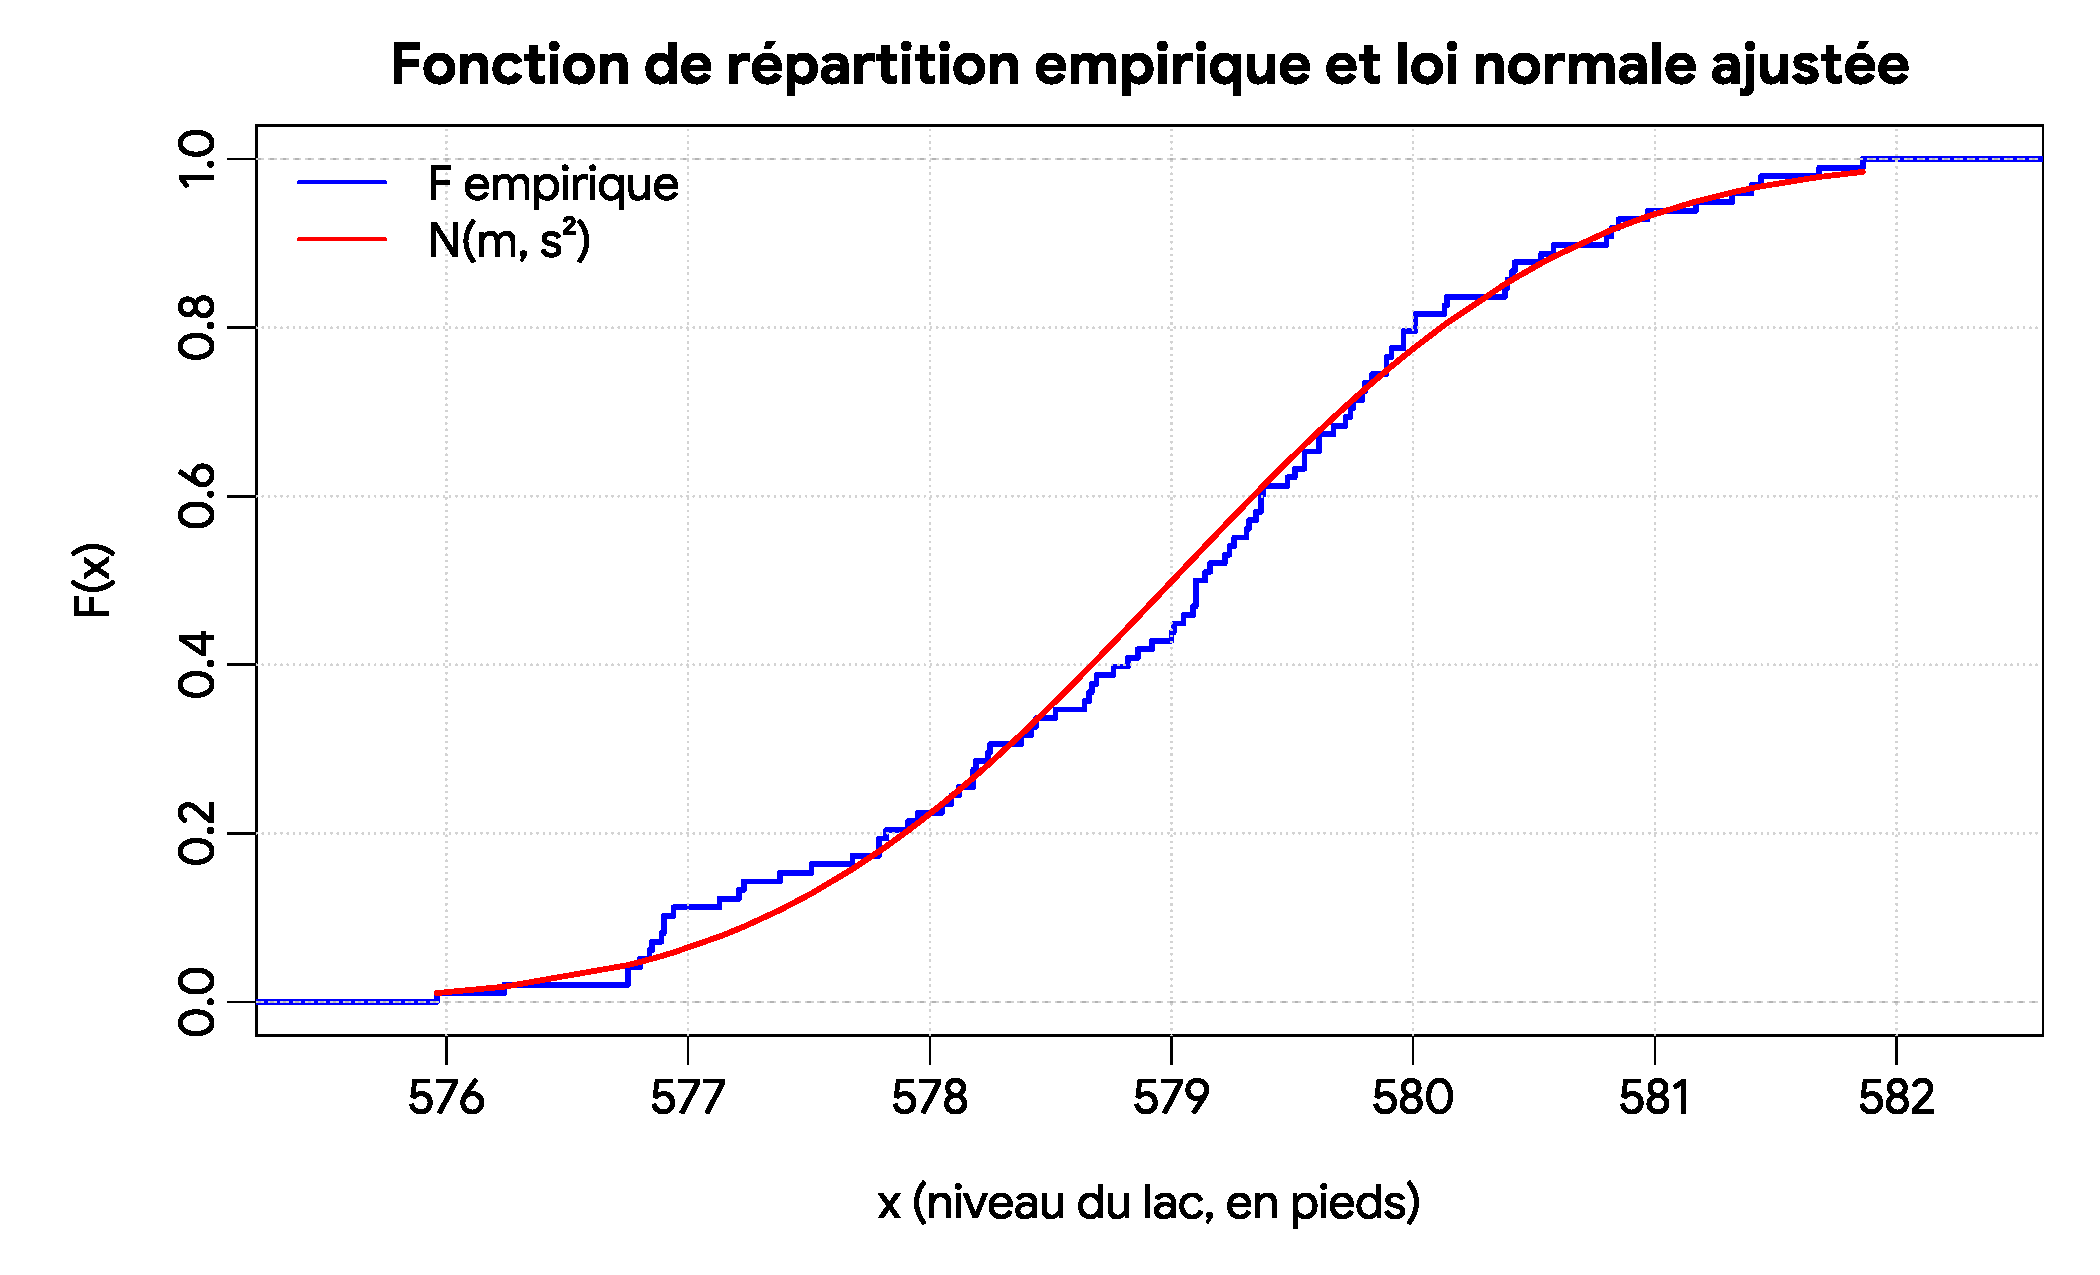
\includegraphics[width=0.82\textwidth]{figures/fig_ecdf.pdf}
\caption{Fonction de répartition empirique de \texttt{Obs}, superposée à celle de la loi $\N(\widehat m,\widehat\sigma^{2})$.}
\label{fig:ecdf}
\end{figure}

Nous remarquons que les deux courbes sont très proches. Les écarts les plus marqués apparaissent dans la queue gauche, vers $577$ pieds (où $F_n>F_0$), puis vers $579$ pieds (où $F_n<F_0$). Ils restent faibles (de l'ordre de $0{,}05$ à $0{,}07$), ce qui suggère que la loi normale ajustée est une approximation raisonnable de la loi des niveaux du lac.

\qst{4. Traçons la fonction quantile empirique et le QQ-plot de la variable \texttt{Obs}.}

\sub{\textbullet\ Traçons la fonction quantile empirique}
La fonction quantile empirique est l'inverse généralisée de la fonction $F_n$ définie précédemment :
\[
  Q_n(p)=\inf\{x : F_n(x)\ge p\}, \qquad p\in(0,1).
\]
Nous l'évaluons sur une grille de $N=1000$ ordres $p$ avec la fonction \texttt{quantile}.

\coder
\begin{codebox}
\begin{lstlisting}
N = 1000
ptx = seq(from = 1/N, to = 1, by = 1/N)
Qn = quantile(Obs, ptx)
plot(ptx, Qn, main = "Fonction quantile empirique",
     xlab = "Ordre p", ylab = "Quantile Qn(p)", col = "blue", pch = 20)
\end{lstlisting}
\end{codebox}

\begin{figure}[H]
\centering
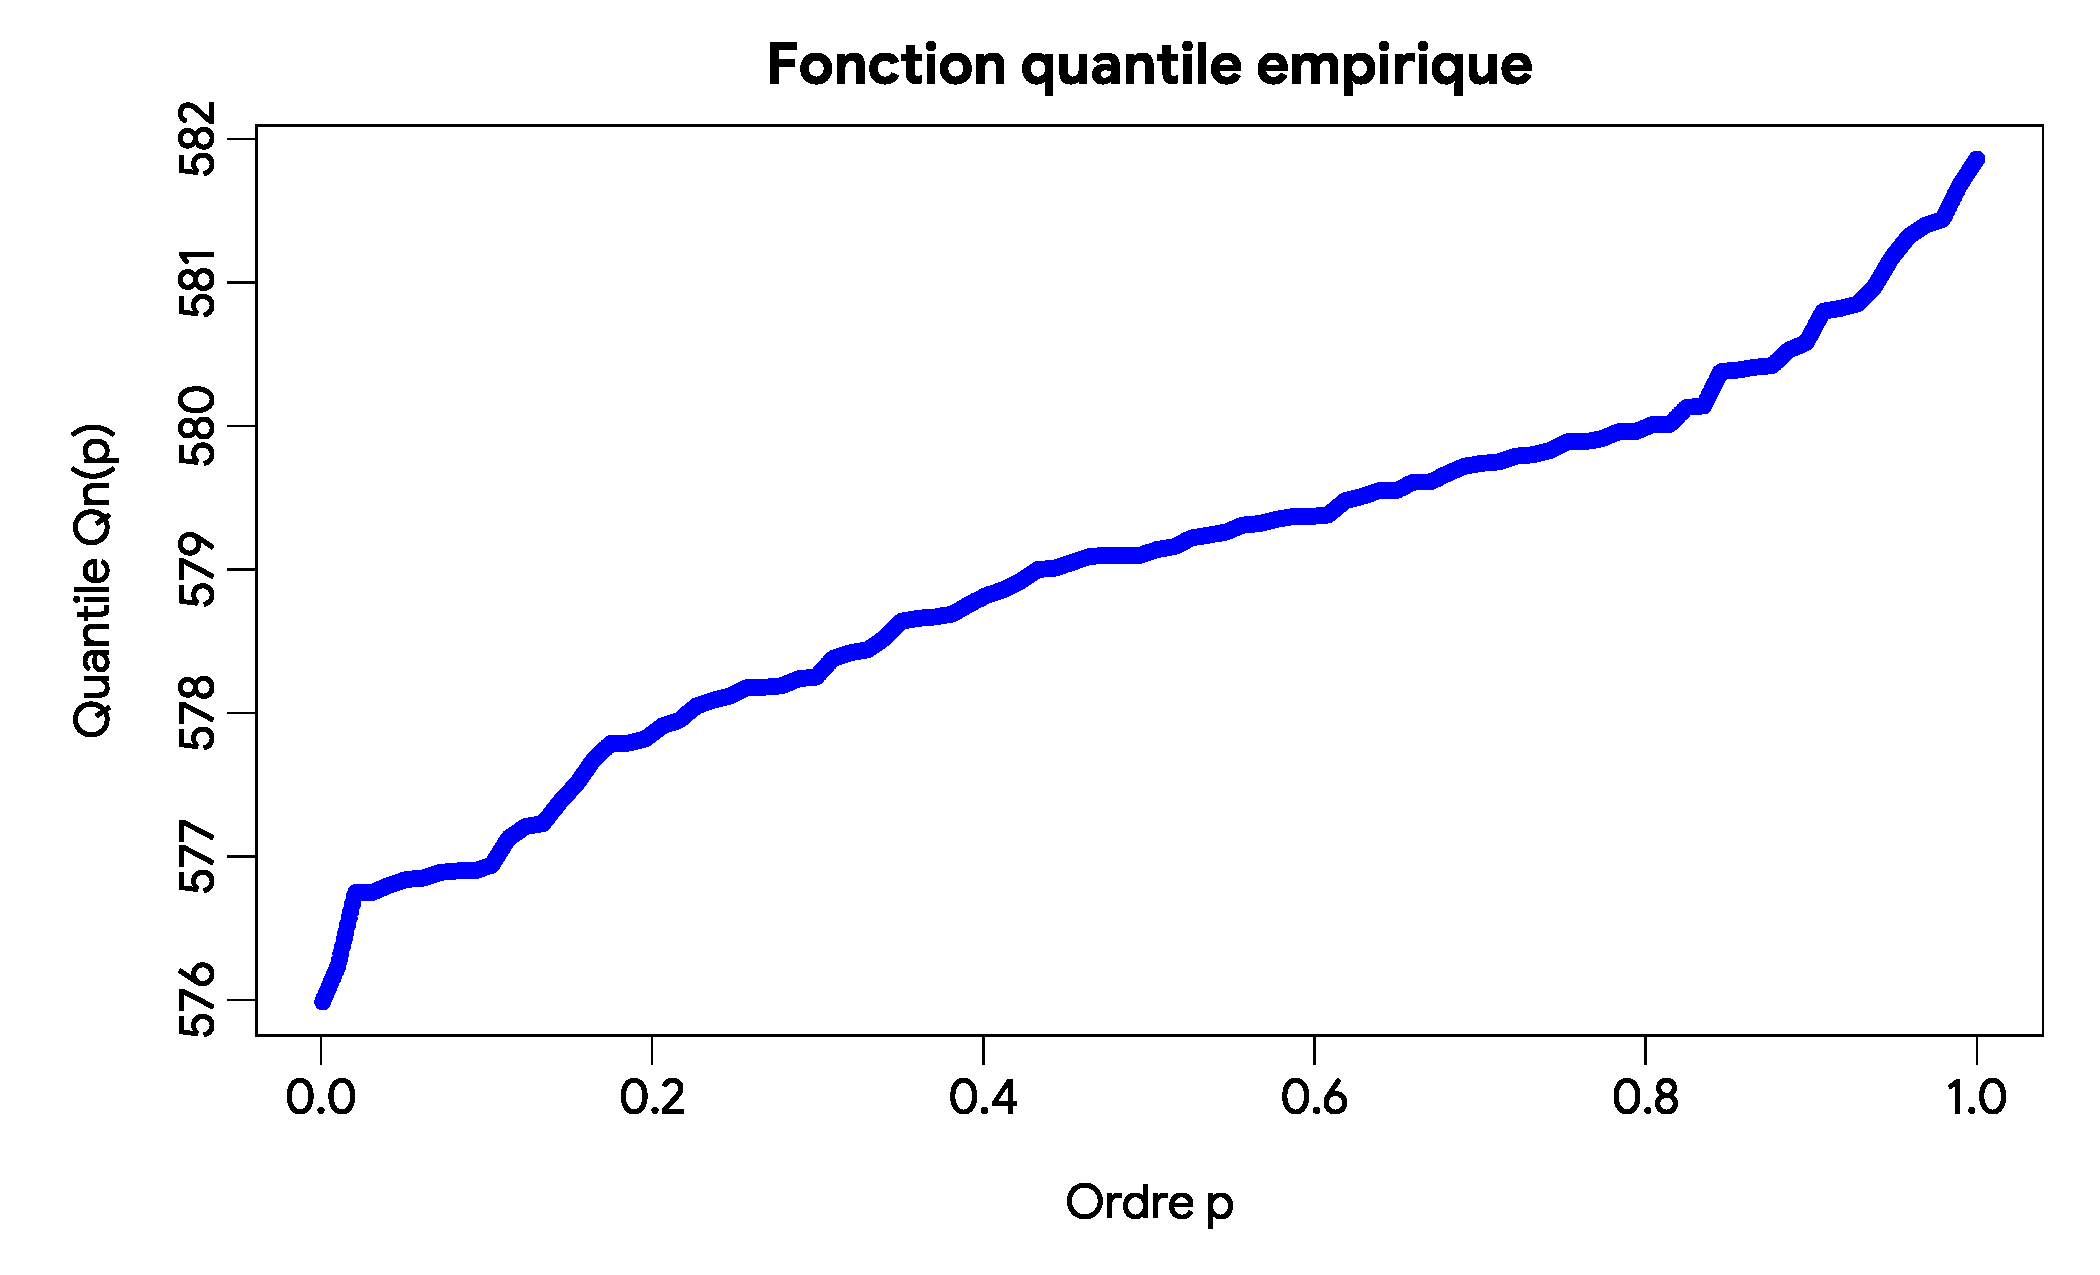
\includegraphics[width=0.82\textwidth]{figures/fig_quant.pdf}
\caption{Fonction quantile empirique de \texttt{Obs}.}
\label{fig:quant}
\end{figure}

On remarque que la fonction quantile est croissante, de $575{,}96$ à $581{,}86$ pieds, avec une médiane d'environ $579{,}1$. De même, sa pente est faible au centre, où les observations sont concentrées, et forte aux extrémités, où les valeurs sont plus dispersées.

\sub{\textbullet\ Traçons maintenant le QQ-plot}

À travers le QQ-plot, on compare les quantiles empiriques aux quantiles théoriques de la loi normale. On représente les points
\[
  \Big(\Phi^{-1}\!\Big(\tfrac{i-1/2}{n}\Big),\ X_{(i)}\Big), \qquad i=1,\dots,n,
\]
où $\Phi$ est la fonction de répartition de la loi $\N(0,1)$. Si les données sont normales, ces points sont proches d'une droite. Sous R, on utilise simplement \texttt{qqnorm} pour tracer les points et \texttt{qqline} pour la droite de référence.

\coder
\begin{codebox}
\begin{lstlisting}
qqnorm(Obs, xlab = "Quantiles théoriques", ylab = "Quantiles empiriques",
       main = "QQ-plot normal", col = "blue", pch = 20)
qqline(Obs, col = "red", lwd = 2)
\end{lstlisting}
\end{codebox}

\begin{figure}[H]
\centering
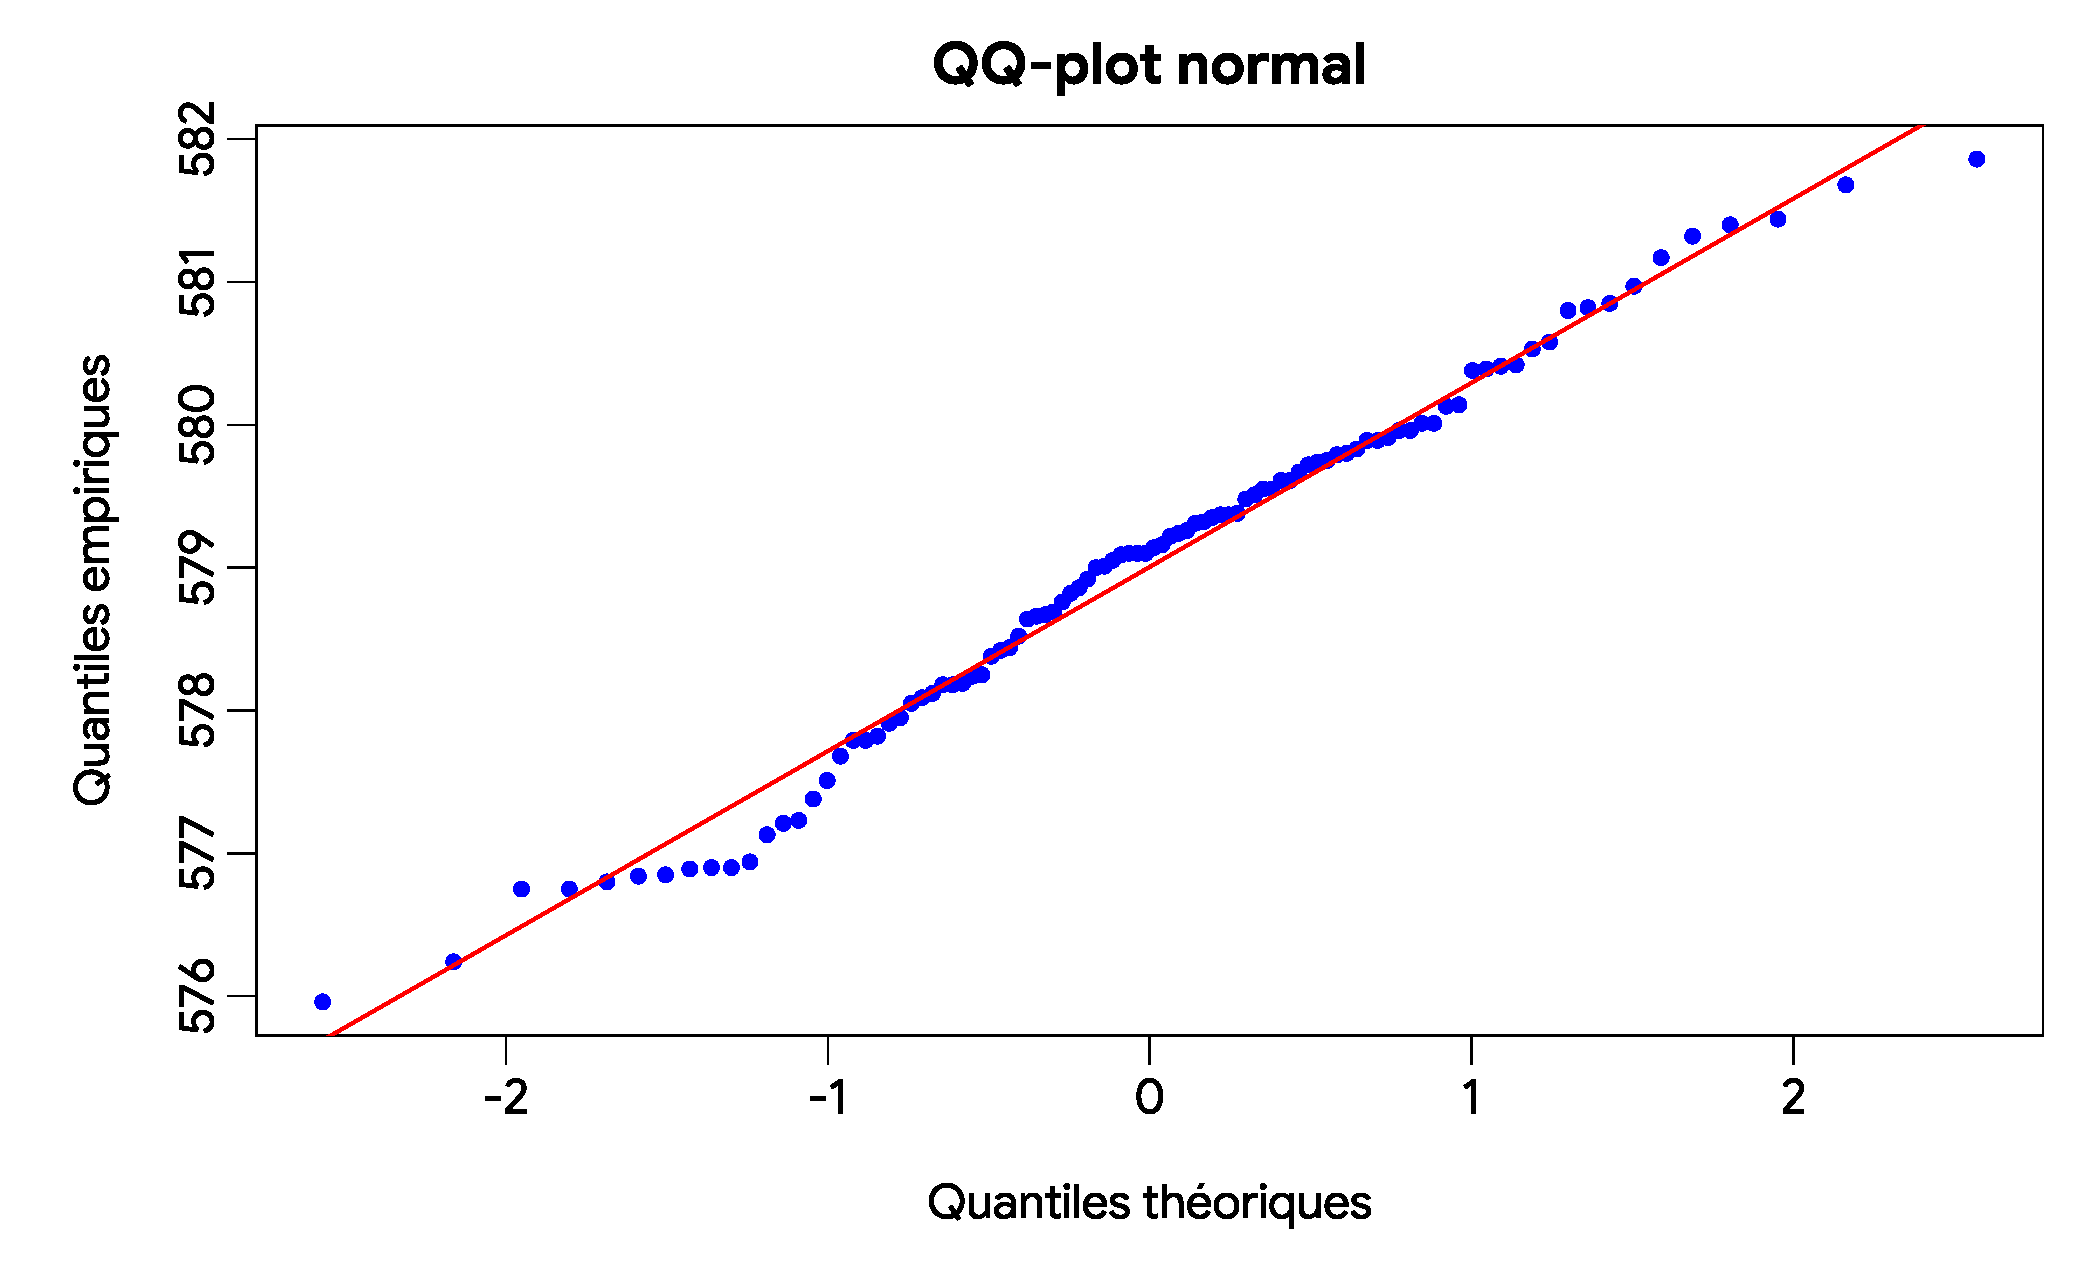
\includegraphics[width=0.82\textwidth]{figures/fig_quant2.pdf}
\caption{QQ-plot normal de \texttt{Obs}.}
\label{fig:qq}
\end{figure}

On remarque que les points du QQ-plot s'alignent bien sur la droite, hormis quelques légers écarts dans la queue gauche, ce qui renforce notre hypothèse de normalité des données.

\qst{5. Traçons l'histogramme et superposons la densité de la loi normale dont l'espérance et l'écart-type sont la moyenne et l'écart-type de la variable \texttt{Obs}.}

Pour tracer cet histogramme, on scinde les données en classes $I_j$ d'amplitude $h_j$ et d'effectif $n_j$. L'histogramme estime la densité par $\widehat f(x)=\dfrac{n_j}{n\,h_j}$ pour $x\in I_j$.
Sous R, nous utilisons la fonction \texttt{hist} avec l'option \texttt{prob = TRUE} pour tracer cette densité (et non les effectifs), ce qui permet la superposition. Par défaut, \texttt{hist} choisit le nombre de classes selon la règle de Sturges, $\lceil 1+\log_2(n)\rceil$.

\coder
\begin{codebox}
\begin{lstlisting}
N = 1000
hist(Obs, prob = TRUE, main = "Histogramme de Obs et densité normale ajustée",
     xlab = "Niveau du lac (en pieds)", ylab = "Densité",
     col = "lightblue", border = "white")
ptx = seq(min(Obs), max(Obs), length = N)
lines(ptx, dnorm(ptx, mean = mean(Obs), sd = sd(Obs)), col = "red", lwd = 2)
\end{lstlisting}
\end{codebox}

\begin{figure}[H]
\centering
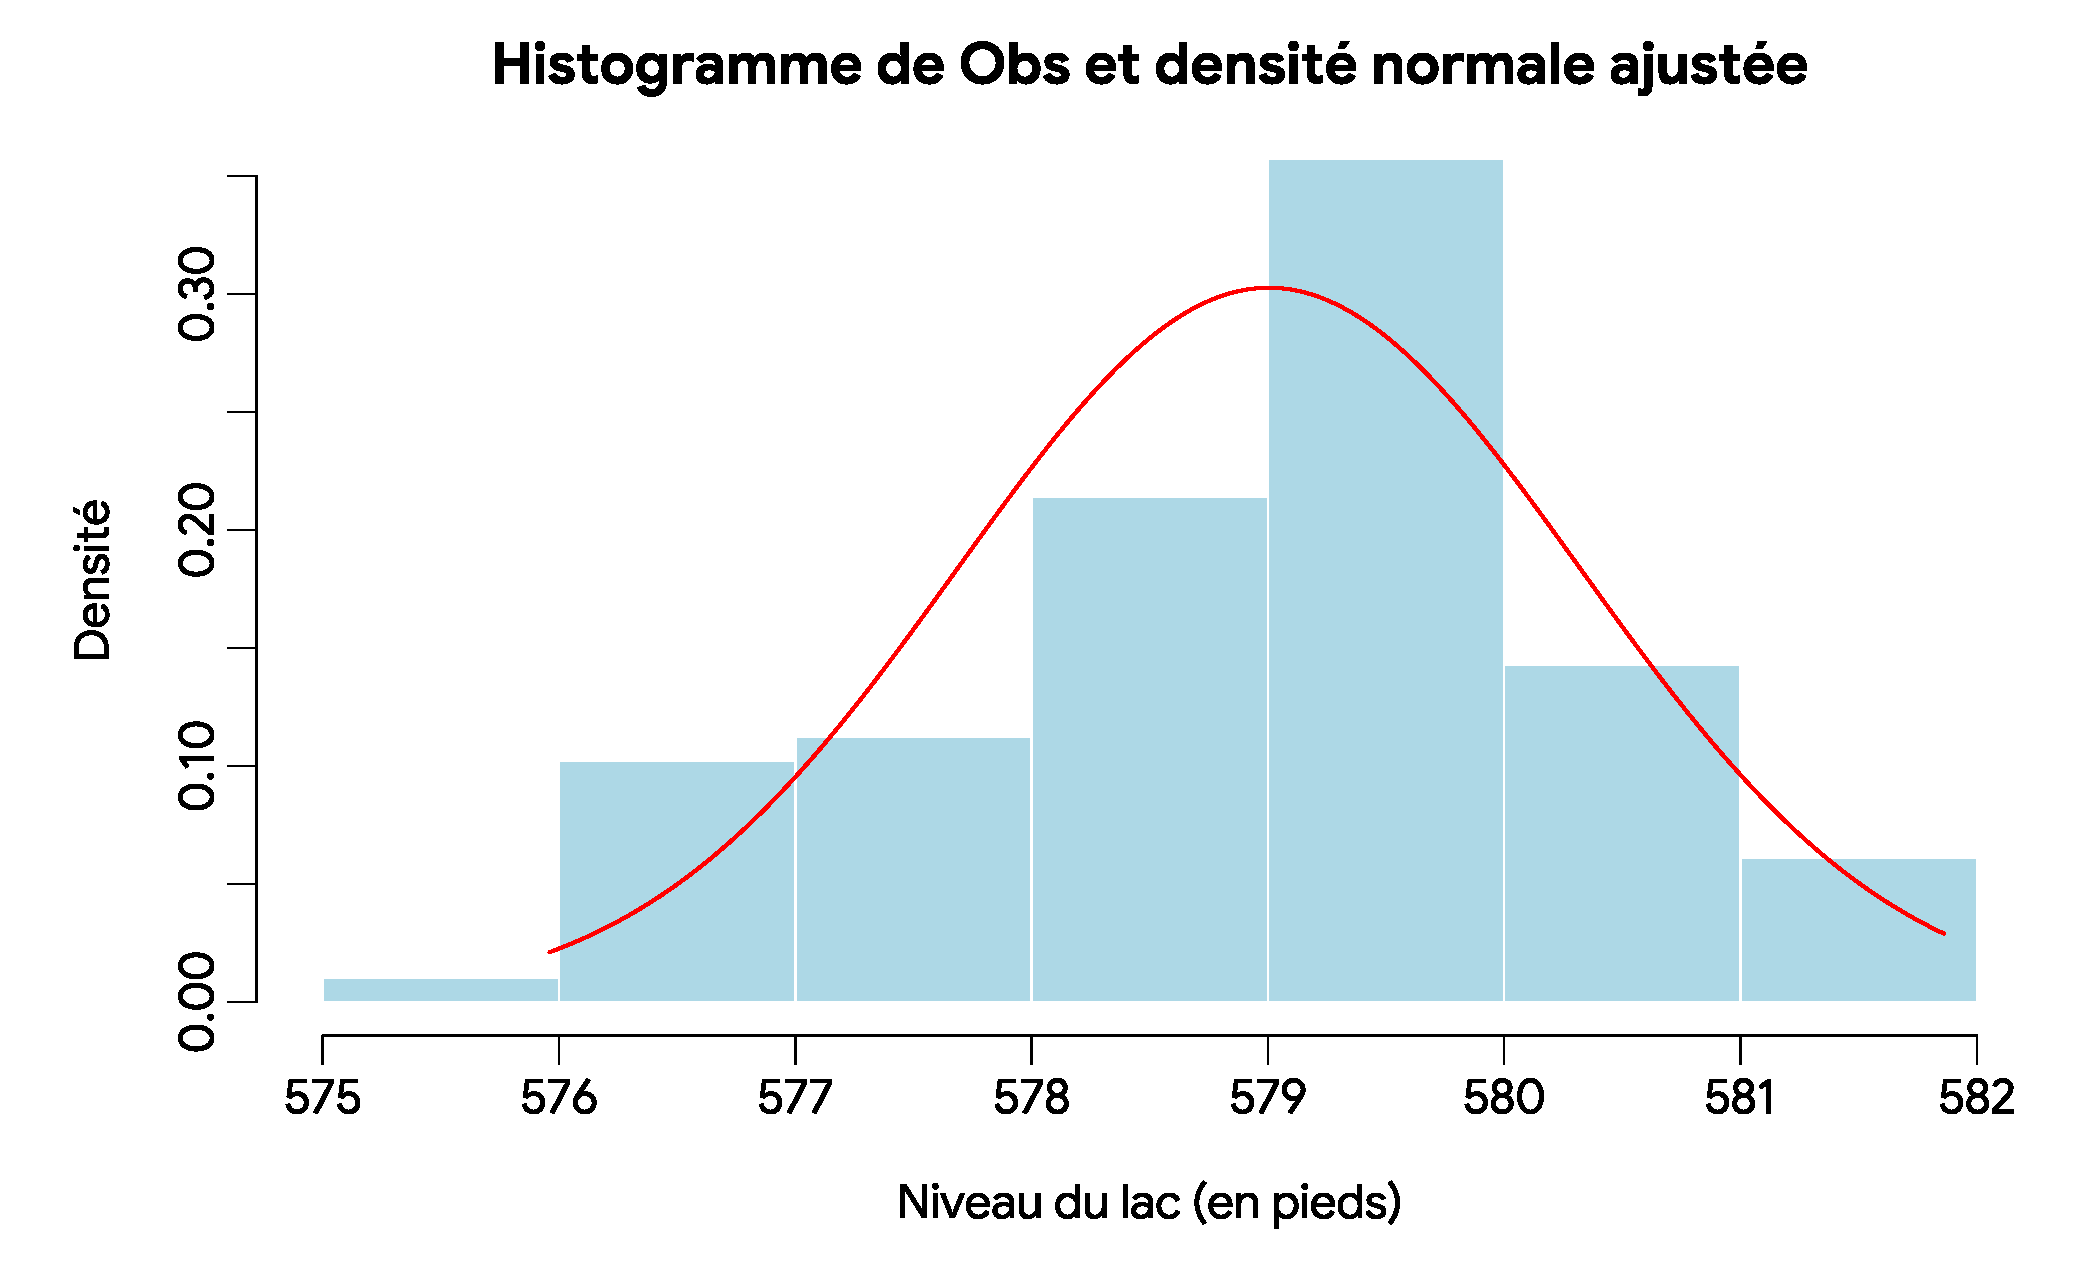
\includegraphics[width=0.82\textwidth]{figures/fig_hist.pdf}
\caption{Histogramme de \texttt{Obs} et densité de la loi $\N(\widehat m,\widehat\sigma^{2})$.}
\end{figure}
L'histogramme est unimodal, avec une classe modale $]579\,;580]$ plus marquée que le pic de la densité normale, et une queue gauche plus étalée, ce qui indique que la loi normale ajustée sous-estime légèrement le pic central et les faibles niveaux.

\qst{6. Calculons puis représentons un estimateur à noyau de la densité.}

L'estimateur à noyau de Parzen--Rosenblatt de la densité est
\[
  \widehat f_h(x)=\frac{1}{nh}\sum_{i=1}^{n}K\!\left(\frac{x-X_i}{h}\right),
\]
où $K$ est le noyau (une densité de probabilité) et $h$ la fenêtre, ou paramètre de lissage. Sous R, on utilise la fonction \texttt{density}, qui propose $7$ noyaux (le noyau gaussien par défaut) et calcule la fenêtre par la règle de Silverman.

\coder
\begin{codebox}
\begin{lstlisting}
dens = density(Obs)
dens$bw
\end{lstlisting}
\end{codebox}

\begin{itemize}[leftmargin=2em, itemsep=2pt]
  \item \textbf{Noyau utilisé : }  Noyau gaussien $K(u)=\frac{1}{\sqrt{2\pi}}e^{-u^{2}/2}$, qui est le noyau par défaut de \texttt{density}.
  \item \textbf{Fenêtre utilisée :}  $h=0{,}4671$, donnée par la règle de Silverman (choix automatique de \texttt{density}) :
  \[ h=0{,}9\,\min\!\big(s,\ \mathrm{IQR}/1{,}34\big)\,n^{-1/5}. \]
\end{itemize}

\sub{\textbullet\ Traçons dans une même fenêtre plusieurs estimateurs à noyau}

On trace dans une même fenêtre graphique les estimateurs obtenus avec les sept noyaux disponibles, en gardant la même fenêtre $h$.

\Needspace{10\baselineskip}
\coder
\begin{codebox}[breakable]
\begin{lstlisting}
kernels = eval(formals(density.default)$kernel)
plot(dens, main = "Estimateurs à noyau de la densité",
     xlab = "Niveau (en pieds)", ylab = "Densité", lwd = 2, ylim = c(0, 0.42))
axis(1, at = seq(575, 583, by = 2))
for (i in 2:length(kernels)) {
  lines(density(Obs, kernel = kernels[i]), col = i, lwd = 2)
}
legend(x = 580.3, y = 0.44, legend = kernels, col = seq(kernels), lty = 1, lwd = 3,
       bty = "n", seg.len = 1, y.intersp = 0.4, x.intersp = 0.4)
\end{lstlisting}
\end{codebox}

\begin{figure}[H]
\centering
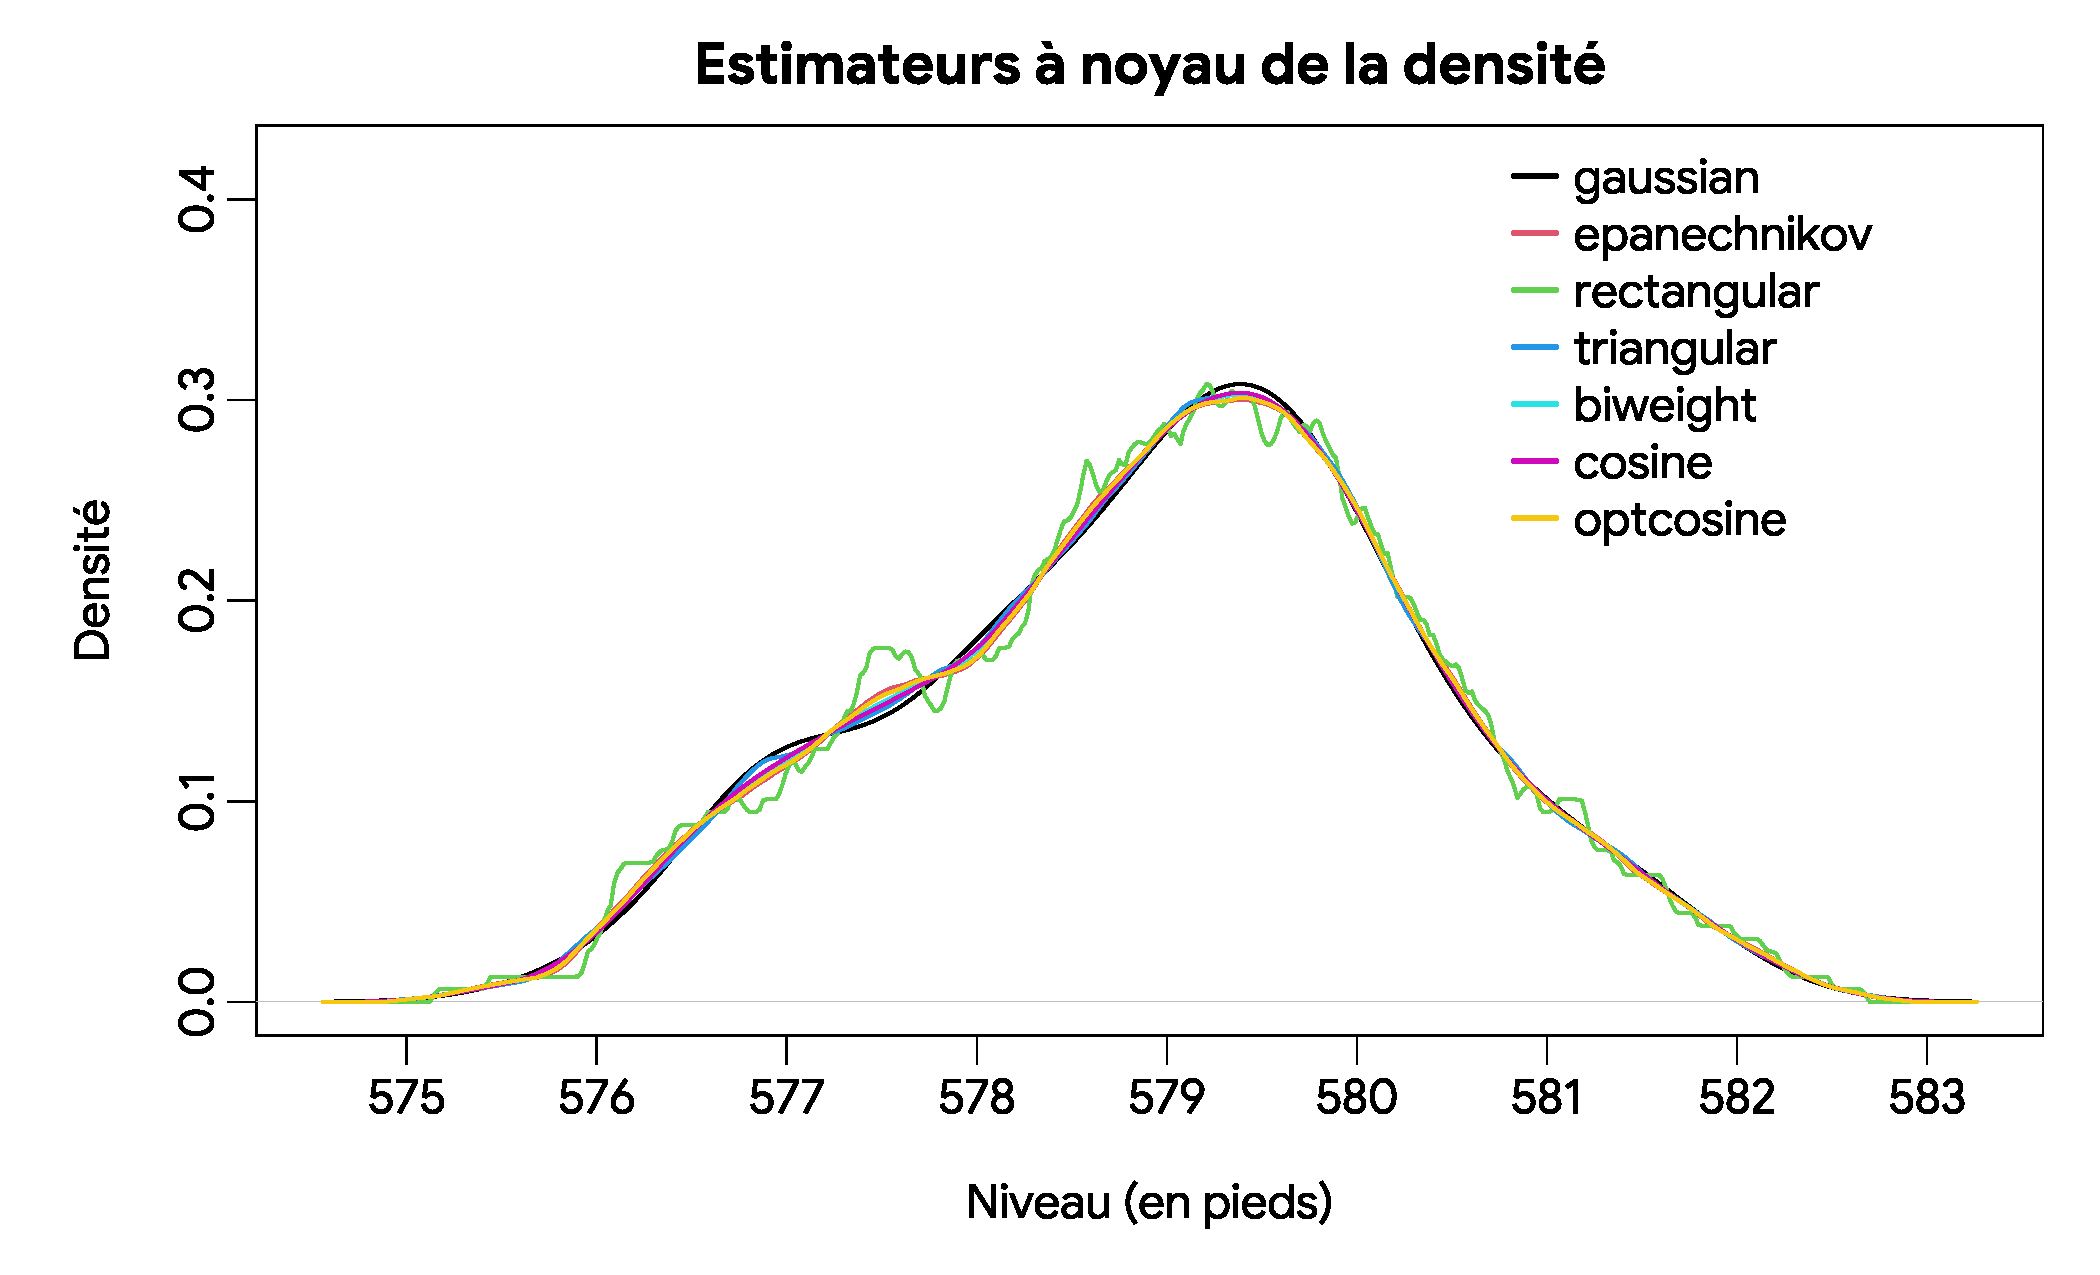
\includegraphics[width=0.82\textwidth]{figures/fig_kernel.pdf}
\caption{Estimateurs à noyau de la densité de \texttt{Obs} pour les sept noyaux de \texttt{density}, avec la même fenêtre $h$.}
\label{fig:noyaux}
\end{figure}

À fenêtre égale ($h=0{,}4671$), les courbes sont presque confondues puisqu'elles ont la même allure, avec un mode voisin de $579{,}3$ pieds et un léger épaulement vers $577$ pieds. Seul le noyau rectangulaire se distingue, car sa courbe est irrégulière, avec de petites oscillations (vers $577{,}5$ et $579{,}5$), ce noyau étant discontinu alors que les autres noyaux, continus, donnent des courbes lisses. \textbf{Le choix du noyau a donc peu d'influence sur l'estimation de la densité.}

\newpage
\section{Estimation par bootstrap}

On dispose de $n=24$ maxima annuels de précipitations journalières (en mm).

\coder
\begin{codebox}
\begin{lstlisting}
x = c(42, 55, 61, 48, 73, 67, 89, 52, 96, 71, 58, 110, 64, 77, 45,
      132, 83, 69, 57, 101, 74, 185, 92, 63)
\end{lstlisting}
\end{codebox}

\qst{1. Calculons la moyenne, la médiane, l'écart-type, les quartiles et le $90^{e}$ percentile empirique.}

\coder
\begin{codebox}
\begin{lstlisting}
moyenne = mean(x)
mediane = median(x)
ecart = sd(x)
quartiles = quantile(x, probs = c(0.25, 0.5, 0.75))
percentile90 = quantile(x, probs = 0.9)
\end{lstlisting}
\end{codebox}

Notons $x_{(1)}\le\dots\le x_{(n)}$ l'échantillon ordonné. Les formules et les fonctions R correspondantes sont rassemblées dans le tableau suivant, avec les valeurs obtenues.

\begin{center}
\renewcommand{\arraystretch}{1.6}
\small
\begin{tabular}{|m{2.3cm}|m{5.9cm}|m{3.4cm}|m{2.2cm}|}
\hline
\textbf{Statistique} & \textbf{Formule} & \textbf{Fonction R} & \textbf{Sortie} \\ \hline
\hhead
Moyenne & $\overline{x}=\dfrac1n\displaystyle\sum_{i=1}^{n}x_i$ & \texttt{mean(x)} & $77{,}67$ \\ \hline
Médiane & $\begin{cases} x_{((n+1)/2)} & \text{si } n \text{ impair}\\[6pt] \dfrac{x_{(n/2)}+x_{(n/2+1)}}{2} & \text{si } n \text{ pair}\end{cases}$\par\vspace{6pt} & \texttt{median(x)} & $70$ \\[9pt] \hline
Écart-type & $s=\sqrt{\dfrac1{n-1}\displaystyle\sum_{i=1}^{n}(x_i-\overline{x})^{2}}$ & \texttt{sd(x)} & $31{,}56$ \\ \hline
Quartiles $Q_1$, $Q_3$ & $Q(p)=x_{(k)}+(h-k)\big(x_{(k+1)}-x_{(k)}\big)$, avec $h=(n-1)p+1$, $k=\lfloor h\rfloor$ ; $p=0{,}25$ et $p=0{,}75$ & \texttt{quantile(x, probs = c(0.25, 0.75))} & $57{,}75$ ; $89{,}75$ \\ \hline
$90^{e}$ percentile & même formule avec $p=0{,}9$ & \texttt{quantile(x, probs = 0.9)} & $107{,}3$ \\ \hline
\end{tabular}
\end{center}

On remarque que la moyenne dépasse la médiane, ce qui indique une asymétrie à droite.

\qst{2. Produisons un histogramme et une boîte à moustaches.}

\coder
\begin{codebox}
\begin{lstlisting}
hist(x, prob = TRUE, main = "Histogramme", xlab = "Précipitation maximale (mm)",
     ylab = "Densité", col = "lightblue", border = "white")
\end{lstlisting}
\end{codebox}

\begin{figure}[!ht]
\centering
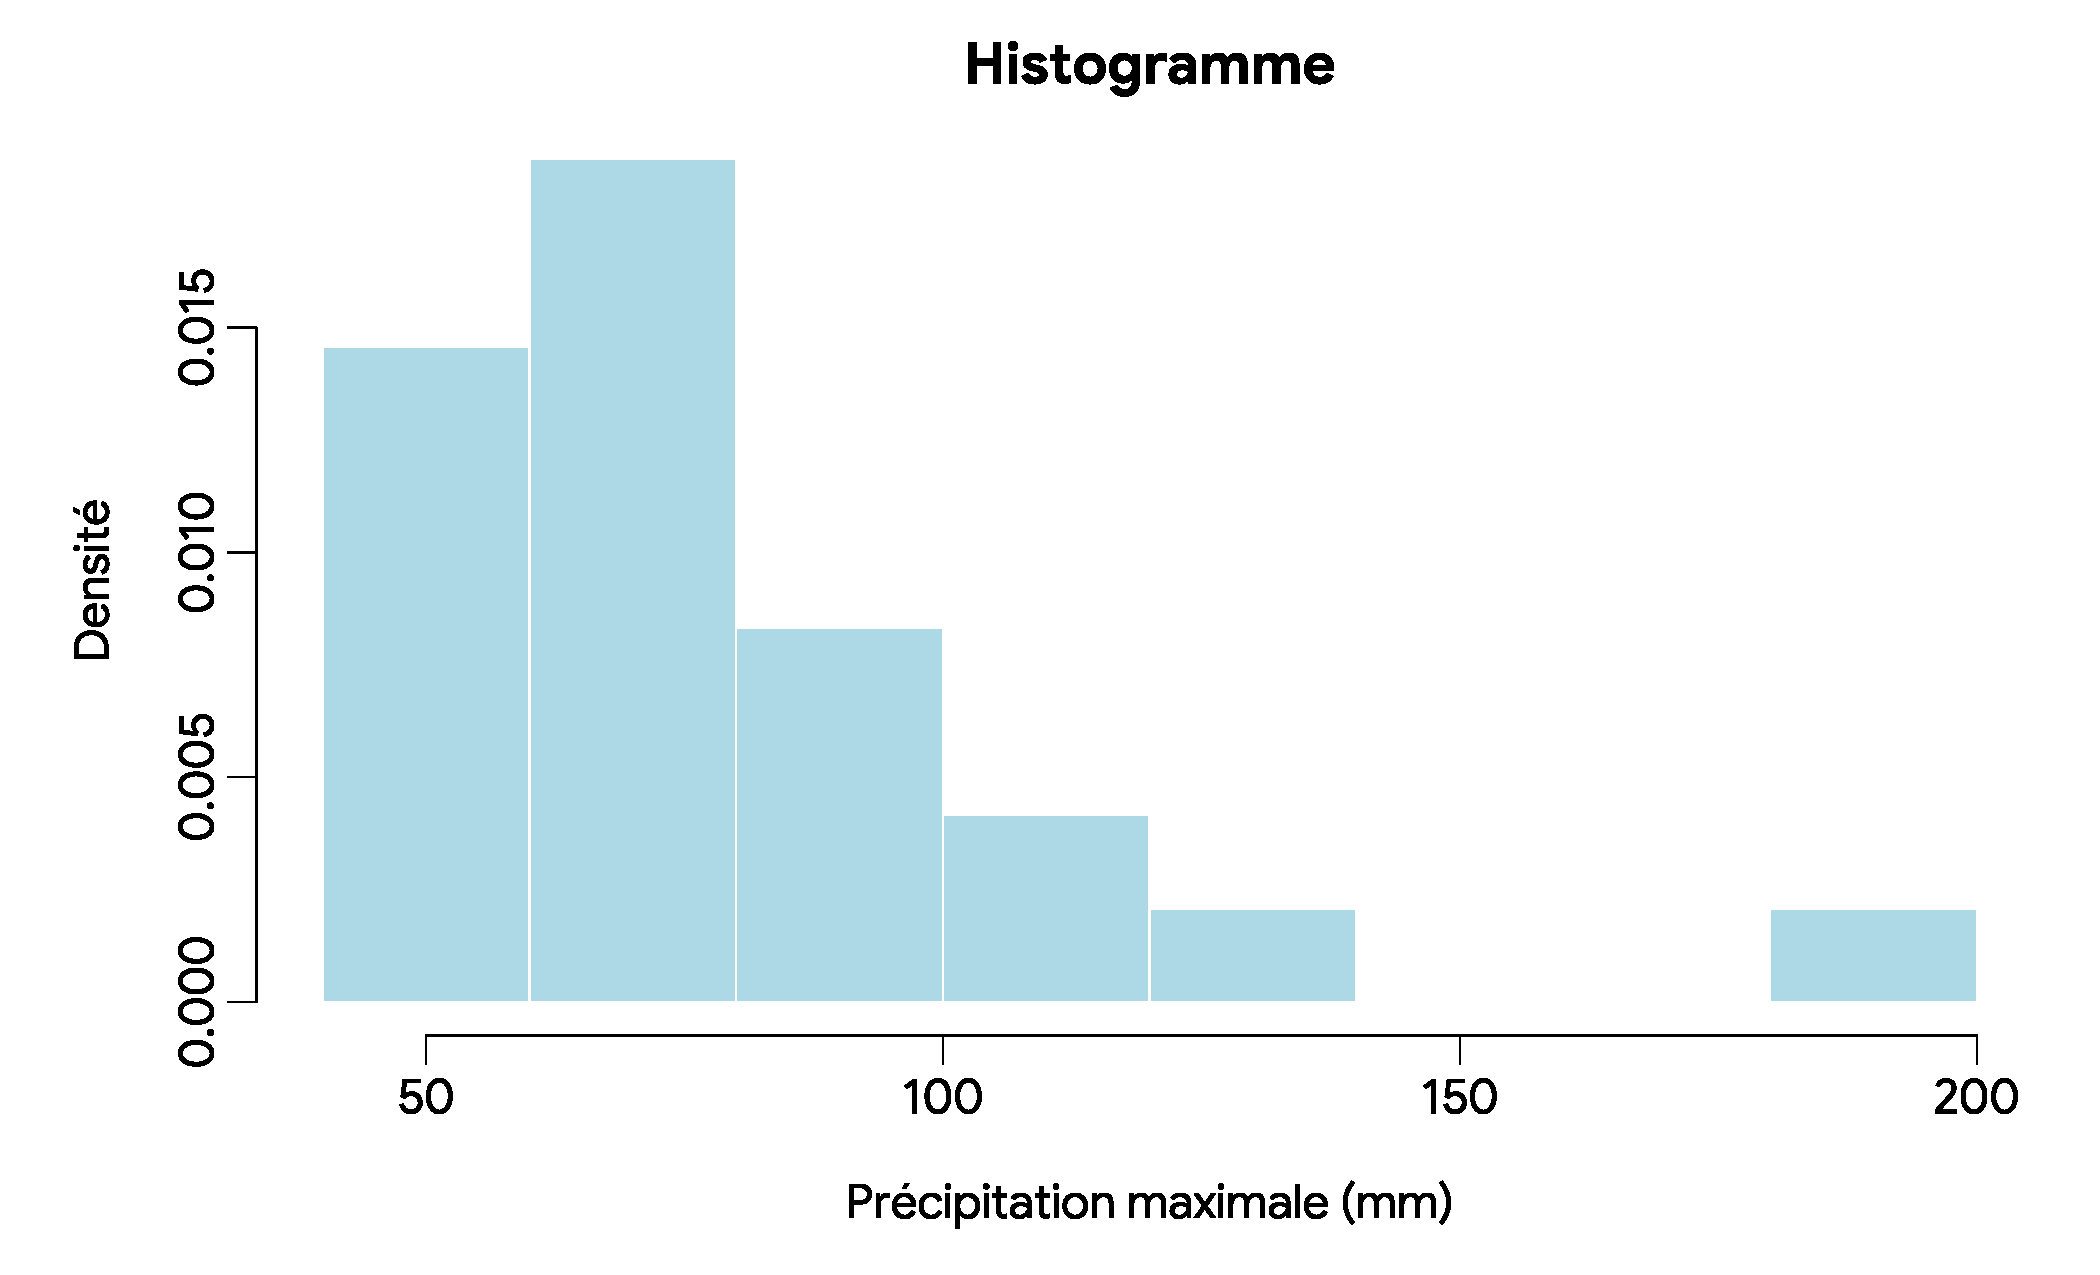
\includegraphics[width=0.7\textwidth]{figures/fig_precip1.pdf}
\caption{Histogramme des maxima annuels de précipitations.}
\label{fig:hist-precip}
\end{figure}

\coder
\begin{codebox}
\begin{lstlisting}
boxplot(x, main = "Boîte à moustaches", ylab = "Précipitation maximale (mm)",
        col = "lightblue")
\end{lstlisting}
\end{codebox}

\begin{figure}[!ht]
\centering
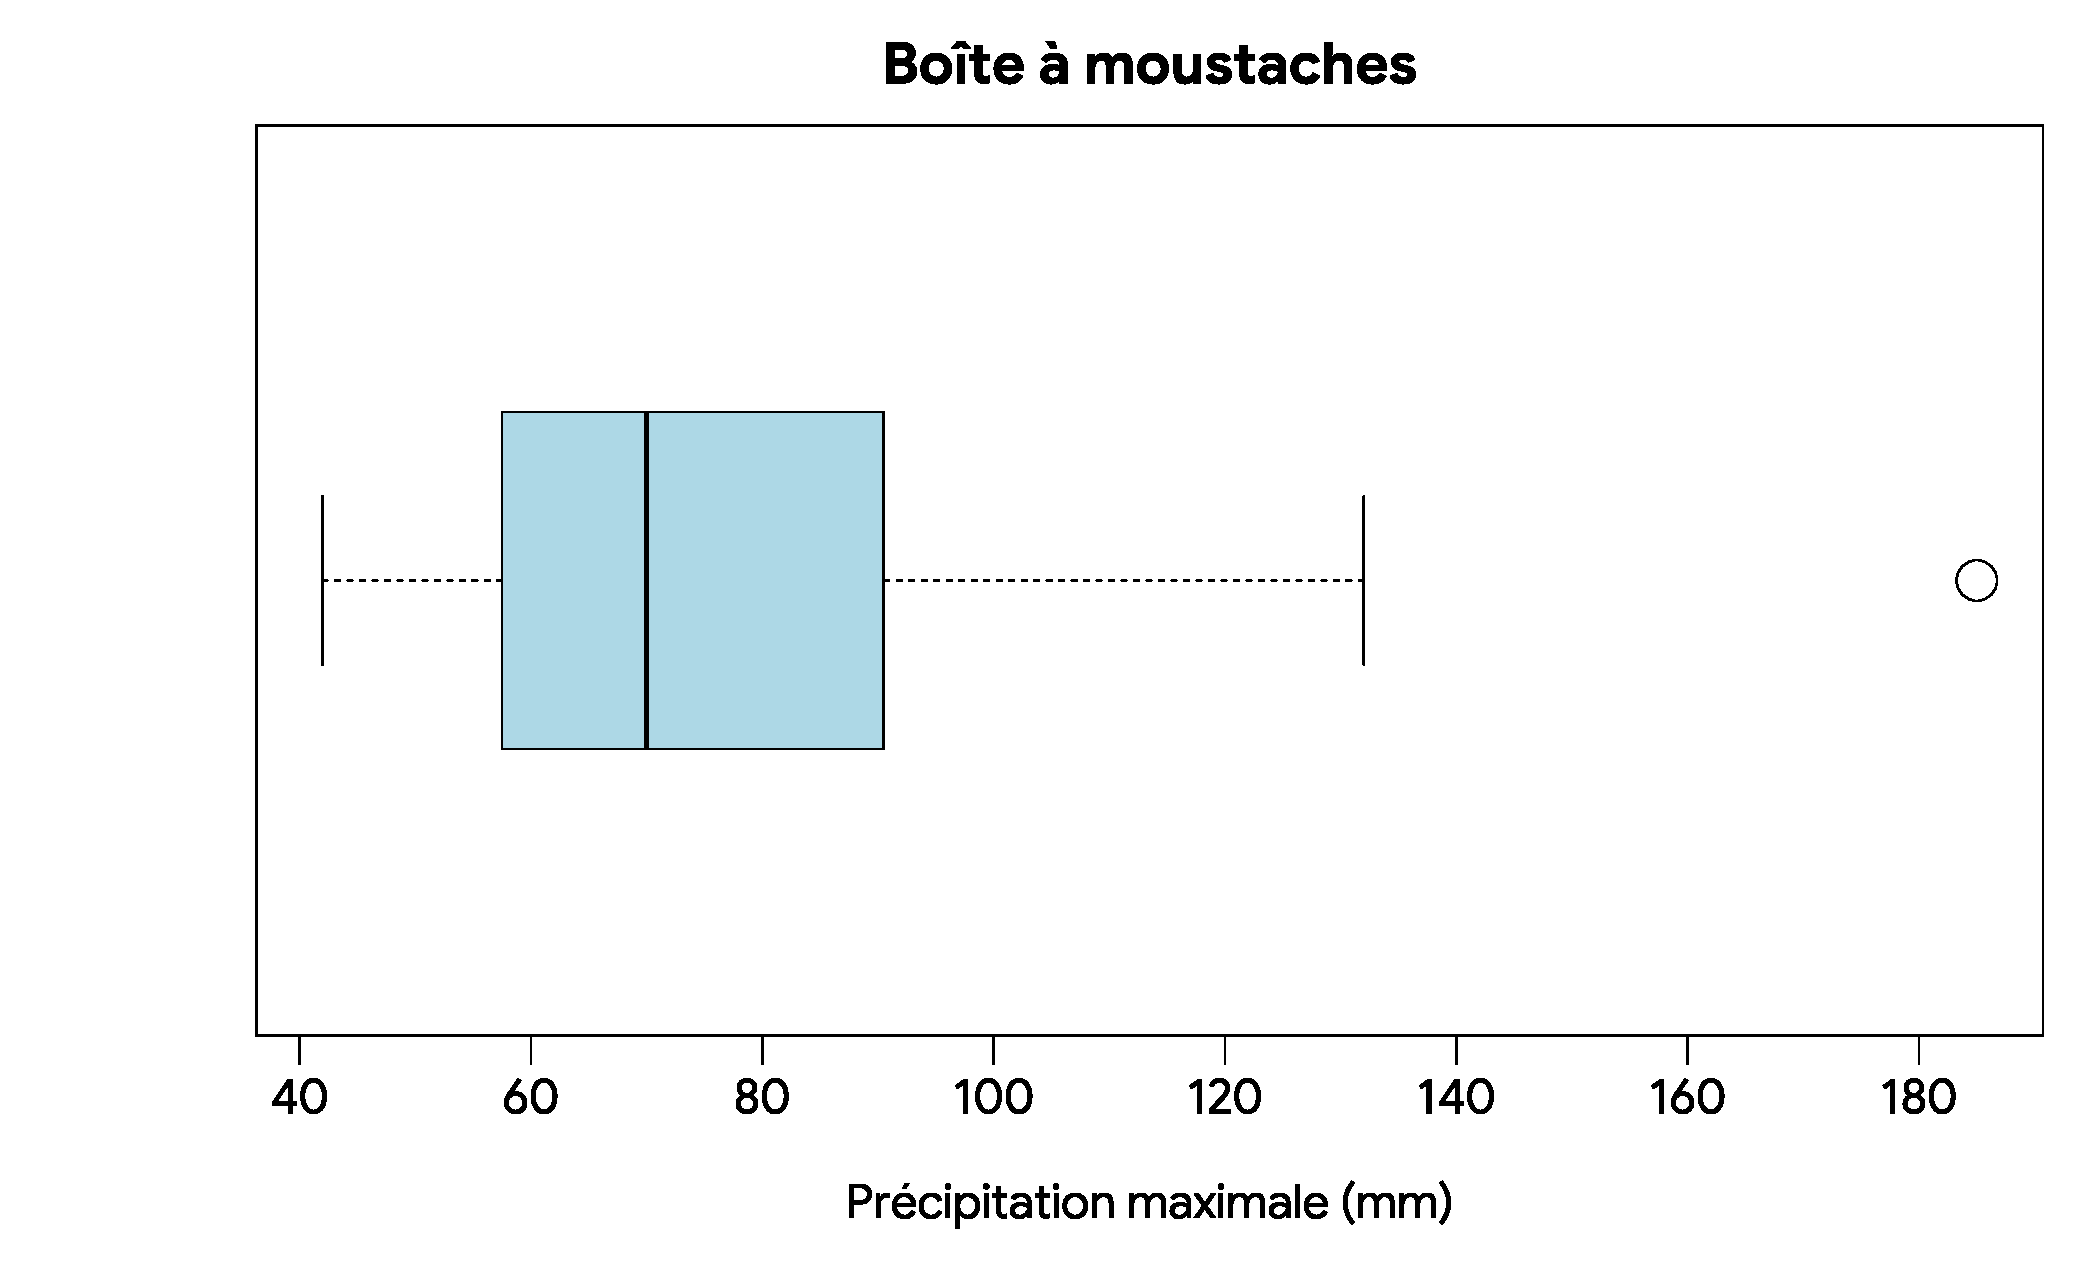
\includegraphics[width=0.75\textwidth]{figures/fig_precip2.pdf}
\caption{Boîte à moustaches des maxima annuels de précipitations.}
\label{fig:box-precip}
\end{figure}

On remarque, d'après l'histogramme et la boîte à moustaches, que la distribution est \textbf{asymétrique à droite}. Par ailleurs, l'écart interquartile vaut $\mathrm{IQR}=32$, d'où la barrière de Tukey $b^{+}=Q_3+1{,}5\,\mathrm{IQR}=137{,}75$. Seule la valeur $185$ mm la dépasse, ce qui en fait une valeur aberrante élevée.

\qst{3. Écrivons une fonction qui réalise $B$ rééchantillonnages bootstrap et calculons, pour chaque échantillon, les trois statistiques suivantes : la moyenne, la médiane et le $90^{e}$ percentile.}

Un échantillon bootstrap est obtenu par $n$ tirages avec remise dans l'échantillon observé. Avec la librairie \texttt{boot}, la définition de ladite fonction devient plus simple.
On a donc :

\coder
\begin{codebox}[breakable]
\begin{lstlisting}
boot_stats <- function(data, indices) {
  xb <- data[indices]
  c(mean(xb), median(xb), quantile(xb, 0.9, names = FALSE))
}
\end{lstlisting}
\end{codebox}
\sub{\textbullet\ Effectuons les calculs pour $B=200$, $1000$, $5000$ et $10000$}

On fixe la graine aléatoire à $123$ avec \texttt{set.seed(123)}. On utilise la fonction R \texttt{lapply} pour appliquer successivement \texttt{boot} à chaque valeur de $B$. Cette dernière nous renvoie une liste de quatre objets de classe \texttt{boot} qu'on nomme selon les valeurs de $B$.

\coder
\begin{codebox}[breakable]
\begin{lstlisting}
library(boot)
set.seed(123)

Bs <- c(200, 1000, 5000, 10000)
sorties <- lapply(Bs, function(B) boot(data = x, statistic = boot_stats, R = B))
names(sorties) <- Bs
sorties
\end{lstlisting}
\end{codebox}

On trouve, pour chaque valeur de $B$, les moyennes bootstrap $\overline{T}^{*}$ de la moyenne, de la médiane et du $90^{e}$ percentile, présentées dans le tableau suivant, avec les valeurs de l'échantillon observé en première ligne :

\begin{center}
\renewcommand{\arraystretch}{1.8}
\begin{tabular}{|c|c|c|c|}
\hline
$\boldsymbol{B}$ & \textbf{Moyenne} & \textbf{Médiane} & $\boldsymbol{90^{e}}$ \textbf{percentile} \\
\hhead
Échantillon observé & $77{,}67$ & $70{,}00$ & $107{,}30$ \\ \hline
$200$    & $77{,}42$ & $70{,}08$ & $111{,}88$ \\ \hline
$1\,000$  & $77{,}27$ & $69{,}65$ & $112{,}01$ \\ \hline
$5\,000$  & $77{,}64$ & $70{,}04$ & $112{,}29$ \\ \hline
$10\,000$ & $77{,}53$ & $69{,}98$ & $111{,}83$ \\ \hline
\end{tabular}
\end{center}
\qst{4. Pour chacune des trois statistiques, calculons le biais bootstrap estimé.}

Pour une statistique $T$, le biais bootstrap estimé est
\[
  \widehat{\mathrm{biais}}_B(T)=\overline{T}^{*}-T(x)=\frac{1}{B}\sum_{b=1}^{B}T_b^{*}-T(x),
\]
où $T_b^{*}$ est la valeur de $T$ sur le $b$-ième échantillon bootstrap et $\overline{T}^{*}$ la moyenne bootstrap.

\coder
\begin{codebox}
\begin{lstlisting}
biais <- t(sapply(sorties, function(res) colMeans(res$t) - res$t0))
colnames(biais) <- c("moyenne", "mediane", "p90")
biais
\end{lstlisting}
\end{codebox}

Les biais obtenus sont donnés dans le tableau suivant :

\begin{center}
\renewcommand{\arraystretch}{1.8}
\begin{tabular}{|c|c|c|c|}
\hline
$\boldsymbol{B}$ & \textbf{Moyenne} & \textbf{Médiane} & $\boldsymbol{90^{e}}$ \textbf{percentile} \\
\hhead
$200$     & $-0{,}2438$ & $0{,}0775$  & $4{,}5840$ \\ \hline
$1\,000$  & $-0{,}3922$ & $-0{,}3515$ & $4{,}7059$ \\ \hline
$5\,000$  & $-0{,}0274$ & $0{,}0374$  & $4{,}9874$ \\ \hline
$10\,000$ & $-0{,}1345$ & $-0{,}0214$ & $4{,}5307$ \\ \hline
\end{tabular}
\end{center}
On pouvait lire directement ces valeurs dans la variable \texttt{sorties}.

On remarque que les biais de la moyenne et de la médiane sont négligeables puisqu'ils restent inférieurs à $0{,}4$ mm en valeur absolue, soit moins de $1\,\%$ de la valeur de la statistique. Par contre, le biais du $90^{e}$ percentile est plus marqué, entre $+4{,}5$ et $+5{,}0$ mm ce qui est lié au fait que ce percentile dépend des plus grandes observations ($132$ et $185$ mm), qui sont peu nombreuses.

\qst{5. Construisons un intervalle de confiance bootstrap à 95\,\% de la médiane par la méthode des quantiles (percentile).}
Sous R, on construit cet intervalle avec la fonction \texttt{boot.ci} et l'option \texttt{type = "perc"}. L'option \texttt{index = 2} désigne la médiane, deuxième statistique de notre fonction \texttt{boot\_stats}. On utilise de nouveau la fonction \texttt{sapply} pour éviter une boucle \texttt{for}.

\coder
\begin{codebox}
\begin{lstlisting}
t(sapply(sorties, function(r) boot.ci(r, conf = 0.95, type = "perc", index = 2)$percent[4:5]))
\end{lstlisting}
\end{codebox}

Les intervalles obtenus sont donnés dans le tableau suivant :

\begin{center}
\renewcommand{\arraystretch}{1.8}
\begin{tabular}{|c|c|c|}
\hline
$\boldsymbol{B}$ & \textbf{Borne inférieure} & \textbf{Borne supérieure} \\
\hhead
$200$     & $61{,}03$ & $83$ \\ \hline
$1\,000$  & $59{,}51$ & $83$ \\ \hline
$5\,000$  & $61$      & $83$ \\ \hline
$10\,000$ & $61$      & $83$ \\ \hline
\end{tabular}
\end{center}
On remarque que la borne inférieure se stabilise à $61$ dès $B=5\,000$, tandis que la borne supérieure reste stable ($83$) quel que soit $B$.

\newpage
\section{Ajustement à la loi normale : données \emph{rivers}}

Le jeu de données \texttt{rivers} contient les longueurs (en miles) de $n=141$ grands fleuves d'Amérique du Nord.

\qst{1. Formulons clairement les hypothèses $H_0$ et $H_1$ du test de Shapiro--Wilk.}

Le test de Shapiro--Wilk permet de tester la normalité d'une distribution. À partir d'un échantillon $X_1,\dots,X_n$, il vérifie si celui-ci peut provenir d'une loi normale $\N(\mu,\sigma^{2})$ dont les paramètres $\mu$ et $\sigma^{2}$ ne sont pas spécifiés. Ainsi, nous pouvons avoir les hypothèses suivantes :
\begin{itemize}[leftmargin=2em, itemsep=2pt]
  \item $H_0$ : l'échantillon est issu d'une loi normale ;
  \item $H_1$ : l'échantillon n'est pas issu d'une loi normale.
\end{itemize}

\qst{2. Exécutons le test sous R, rapportons la statistique, la $p$-valeur et la décision au seuil de $5\,\%$.}

\coder
\begin{codebox}
\begin{lstlisting}
data(rivers)
result = shapiro.test(rivers)
result$statistic
result$p.value
\end{lstlisting}
\end{codebox}
On trouve \quad \resbox{$W=0{,}6666$}\quad \text{et} \quad \resbox{$p\text{-valeur}=\num{1.869e-16}$}

Comme $p\text{-valeur}<0{,}05$, on rejette $H_0$ au seuil de $5\,\%$. Ainsi, au risque de $5\,\%$, on conclut que l'échantillon n'est pas issu d'une loi normale.

\qst{3. Effectuons un test de Kolmogorov--Smirnov et expliquons les conditions d'application de sa version classique.}

Le test de Kolmogorov--Smirnov vérifie si un échantillon $X_1,\dots,X_n$ de fonction de répartition inconnue $F$ suit une loi $F_0$ donnée :
\[
  H_0 : F=F_0 \qquad\text{contre}\qquad H_1 : F\neq F_0 .
\]
Dans notre cas, $F_0$ est la fonction de répartition de la loi normale de paramètres $\overline{x}$ et $s$, avec
\[
  \overline{x}=\frac{1}{n}\sum_{i=1}^{n}x_i \qquad \text{ et }
  \qquad
  s=\sqrt{\frac{1}{n-1}\sum_{i=1}^{n}\big(x_i-\overline{x}\big)^{2}} .
\]
Sous R, nous utilisons la fonction \texttt{ks.test}.

\coder
\begin{codebox}
\begin{lstlisting}
result = ks.test(rivers, "pnorm", mean = mean(rivers), sd = sd(rivers))
result
\end{lstlisting}
\end{codebox}
On trouve \quad \resbox{$D=0{,}2082$}\quad \text{et} \quad \resbox{$p\text{-valeur}=\num{9.768e-6}$}

Comme $p\text{-valeur}<0{,}05$, on rejette $H_0$ au seuil de $5\,\%$.

\sub{Conditions d'application de la version classique}

La version classique du test de Kolmogorov--Smirnov suppose que :
\begin{itemize}[leftmargin=2em, itemsep=2pt]
  \item les observations sont indépendantes et identiquement distribuées ;
  \item la loi $F_0$ est continue et entièrement spécifiée avant l'observation des données, c'est-à-dire que ses paramètres sont connus et non estimés sur l'échantillon ;
  \item il n'y a pas d'ex æquo.
\end{itemize}

Dans notre cas, $\mu$ et $\sigma$ sont estimés et l'échantillon contient des ex æquo ($114$ valeurs distinctes sur $141$), ce que \texttt{ks.test} signale par un avertissement. L'estimation des paramètres rend le test conservateur car la vraie $p$-valeur est plus petite que celle affichée. Le rejet de $H_0$ reste donc valable.

\qst{4. À partir des tests, concluons sur la plausibilité du modèle normal.}

Les deux tests rejettent la normalité, avec des $p$-valeurs très inférieures à $0{,}05$. De plus, la moyenne ($591{,}2$) est nettement supérieure à la médiane ($425$), signe d'une forte asymétrie à droite. \\[1cm]
D'où \quad \resboxl{Le modèle normal n'est pas plausible pour les longueurs des fleuves d'Amérique du Nord.}

\newpage
\section{Comparaison de mesures appariées et choix du test}

On note $X_1$ le nombre de bactéries par cm\textsuperscript{3} juste après la traite et $X_2$ celui mesuré $24$ h plus tard, pour $n=8$ vaches.

\coder
\begin{codebox}
\begin{lstlisting}
juste_apres_traite <- c(12000, 13000, 21500, 17000, 15000, 22000, 11000, 21000)
apres_24h          <- c(11000, 20000, 31000, 28000, 26000, 30000, 16000, 29000)
\end{lstlisting}
\end{codebox}

\qst{1. Définissons la variable de réponse}

La variable de réponse est \textbf{le nombre de bactéries par cm\textsuperscript{3} de lait.}

\sub{\textbullet\ Construisons le vecteur des différences $D=(\text{mesure à }24\text{ h}-\text{mesure juste après la traite})$.}
 On pose $D_i=X_{2,i}-X_{1,i}$.

\coder
\begin{codebox}
\begin{lstlisting}
D <- apres_24h - juste_apres_traite
D
\end{lstlisting}
\end{codebox}
Les sorties se présentent comme suit :
\begin{center}
\renewcommand{\arraystretch}{1.8}
\small
\begin{tabular}{|c|c|c|c|c|c|c|c|c|}
\hline
\textbf{Vache} & \textbf{1} & \textbf{2} & \textbf{3} & \textbf{4} & \textbf{5} & \textbf{6} & \textbf{7} & \textbf{8} \\
\hhead
$X_1$ & $12\,000$ & $13\,000$ & $21\,500$ & $17\,000$ & $15\,000$ & $22\,000$ & $11\,000$ & $21\,000$ \\ \hline
$X_2$ & $11\,000$ & $20\,000$ & $31\,000$ & $28\,000$ & $26\,000$ & $30\,000$ & $16\,000$ & $29\,000$ \\ \hline
$D$   & $-1\,000$ & $7\,000$ & $9\,500$ & $11\,000$ & $11\,000$ & $8\,000$ & $5\,000$ & $8\,000$ \\ \hline
\end{tabular}
\end{center}

\sub{\textbullet\ Expliquons pourquoi la structure des données est appariée.}

La structure des données est appariée car les deux mesures d'une même ligne portent sur la même vache et ne sont donc pas indépendantes.

\qst{2. Sous l'hypothèse que les différences suivent une loi normale, effectuons un test $t$ apparié.}
Les deux hypothèses qu'on teste sont :
\[
  H_0 : \mu_D=0 \qquad\text{contre}\qquad H_1 : \mu_D>0 ,
\]
où $\mu_D=\E(D)$ désigne l'espérance de la différence $D$, c'est-à-dire l'augmentation moyenne du nombre de bactéries par cm\textsuperscript{3} entre la traite et $24$ h après.\\ Sous $H_0$, il n'y a pas d'augmentation moyenne et sous $H_1$, le nombre de bactéries augmente en moyenne.

Dans R, on utilise la fonction \texttt{t.test}.
\coder
\begin{codebox}
\begin{lstlisting}
result = t.test(apres_24h, juste_apres_traite, paired = TRUE, alternative = "greater")
print(result)
IC = t.test(apres_24h, juste_apres_traite, paired = TRUE)$conf.int
print(IC)
\end{lstlisting}
\end{codebox}
Le second appel, sans l'option \texttt{alternative}, fournit l'intervalle de confiance bilatéral. On trouve donc :
\begin{center}
\resbox{$t=5{,}2786$} \quad
\resbox{$\mathrm{df}=7$} \quad
\resbox{$p\text{-valeur}=\num{5.749e-4}$} \\[10pt]
\resbox{$\overline{D}=7\,312{,}5$} \quad \text{ et }  \quad
\resbox{$\mathrm{IC}_{95\,\%}(\mu_D)=[\,4\,036{,}8\ ;\ 10\,588{,}2\,]$}
\end{center}
On remarque que $p\text{-valeur}=\num{5.749e-4}<0{,}05$, donc on rejette $H_0$ au risque de $5\,\%$.

\qst{3. Effectuons un test du signe unilatéral sur les différences.}

Le test du signe nous permet de tester si la médiane des différences $D$ est nulle, en n'utilisant que le signe de chaque $D_i$.

Les hypothèses testées sont :
\[
  H_0 : \operatorname{med}(D)=0 \quad(\text{soit } \P(D>0)=\tfrac12) \qquad\text{contre}\qquad H_1 : \operatorname{med}(D)>0 \quad(\text{soit } \P(D>0)>\tfrac12).
\]
Sous $H_0$, le nombre $S$ de différences positives suit une loi binomiale $\mathcal B(n,\tfrac12)$.

Sous R, on utilise la fonction \texttt{binom.test}.

\coder
\begin{codebox}
\begin{lstlisting}
plus  <- sum(D > 0)
moins <- sum(D < 0)
n     <- plus + moins
binom.test(plus, n = n, p = 0.5, alternative = "greater")
\end{lstlisting}
\end{codebox}

On observe $S=7$ différences positives sur $8$ et la $p$-valeur vaut $0{,}03516$.

Comme $p\text{-valeur}<0{,}05$, on rejette $H_0$ au seuil de $5\,\%$.

\sub{\textbullet\ Expliquons ce que ce test suppose (et ne suppose pas) sur la distribution des différences.}
Ce test suppose seulement que les $D_i$ sont indépendants et de même loi, avec $\P(D=0)=0$ pour que la médiane soit bien définie. Il ne suppose ni la normalité, ni la symétrie de la distribution des différences. Il ne teste que la médiane de $D$.

\qst{4. Effectuons un test de Wilcoxon pour données appariées (test des rangs signés).}

Le test de Wilcoxon des rangs signés nous permet de tester si les différences $D$ sont centrées en $0$, en utilisant à la fois leur signe et le rang de leur valeur absolue.
La statistique $V$ est la somme des rangs des $|D_i|$ associés aux différences positives. Les hypothèses testées sont :
\[
  \begin{aligned} H_0 &: \text{la distribution de } D \text{ est symétrique et centrée en } 0,\\ H_1 &: \text{la distribution de } D \text{ est symétrique et centrée en une valeur } >0. \end{aligned}
\]
Contrairement au test du signe, ce test suppose donc que la distribution de $D$ est \emph{symétrique} autour de sa médiane.

Sous R, on utilise la fonction \texttt{wilcox.test}.

\coder
\begin{codebox}
\begin{lstlisting}
wilcox.test(apres_24h, juste_apres_traite, paired = TRUE, alternative = "greater", exact = FALSE)
\end{lstlisting}
\end{codebox}

On trouve \quad \resbox{$V=35$} \quad et \quad \resbox{$p\text{-valeur}=0{,}0103$}

Nous utilisons \texttt{exact = FALSE} car $D$ contient des ex æquo en valeur absolue ($8\,000$ et $11\,000$ apparaissent chacun deux fois), ce qui empêche le calcul exact de la loi de $V$ : \texttt{R} utilise alors l'approximation normale avec correction de continuité.

Comme $p\text{-valeur}<0{,}05$, on rejette $H_0$ au seuil de $5\,\%$.

\sub{\textbullet\ Comparons les trois méthodes}

\begin{center}
\renewcommand{\arraystretch}{1.8}
\begin{tabular}{|l|c|c|c|c|}
\hline
\textbf{Test} & \textbf{Statistique} & $\boldsymbol{p}$\textbf{-valeur} & \textbf{Décision à} $\boldsymbol{5\,\%}$ & \textbf{Décision à} $\boldsymbol{1\,\%}$ \\
\hhead
$t$ apparié & $t=5{,}2786$ & $\num{5.749e-4}$ & rejet & rejet \\ \hline
Signe       & $S=7$        & $0{,}0352$       & rejet & non-rejet \\ \hline
Wilcoxon    & $V=35$       & $0{,}0103$       & rejet & non-rejet \\ \hline
\end{tabular}
\end{center}
Le tableau montre que les trois tests conduisent au rejet de $H_0$ au seuil de $5\,\%$. \\[1cm]
D'où \quad \resboxl{Au seuil de $5\,\%$, le nombre de bactéries par cm\textsuperscript{3} augmente significativement en $24$ heures.}

\bigskip
\begin{res}
\centering\hyphenpenalty=10000\exhyphenpenalty=10000
\textbf{Code source.} L'ensemble de nos codes R a été structuré et enregistré sur le dépôt GitHub suivant :\\[4pt]
\href{https://github.com/Parfait0123/Simulation-Aleatoire-2}{\texttt{https://github.com/Parfait0123/Simulation-Aleatoire-2}}
\end{res}

\end{document}
